 %!TEX root = ./template-skripsi.tex
%-------------------------------------------------------------------------------
%                            BAB II
%               KAJIAN TEORI
%-------------------------------------------------------------------------------

\chapter{KAJIAN PUSTAKA} 

\section{\textit{Search Engine}}
\textit{Search Engine} merupakan sebuah perangkat lunak yang dirancang untuk mencari informasi dalam \textit{internet}. Dalam penggunaannya, pengguna memasukan kata kunci yang ingin pengguna cari dalam \textit{search engine} dan \textit{search engine} akan menampilkan daftar dokumen, suara, gambar, \textit{video} dan lain lain yang relevan dengan kata kunci yang pengguna masukkan.

\textit{Search engine} menggunakan sebuah perangkat lunak bernama \textit{crawler} yang bertugas untuk memindai dan meng-\textit{index} halaman \textit{web} yang berada di \textit{internet}. \textit{Crawler} ini mengikuti tautan dari satu halaman ke halaman lainnya mengumpulkan informasi mengenai konten dan struktur \textit{website}. Data yang berhasil dikumpulkan tersebut lalu disimpan dalam sebuah \textit{database} yang membentuk \textit{search engine} index. Beberapa contoh \textit{search engine} yang populer pada saat ini adalah Google, Yahoo, Bing, Baidu dan Yandex.


\section{\textit{Agile}}
Pengembangan perangkat lunak menggunakan \textit{agile} merupakan salah satu metode pengembangan perangkat lunak yang ada. Kata "\textit{agile}" memiliki arti cepat, ringan dan bebas bergerak. Konsep pengembangan perangkat lunak menggunakan \textit{agile} ditemukan oleh Kent Beck dan 16 koleganya dengan menyatakan \textit{agile} adalah cara dalam membangun sebuah perangkat lunak dengan cara mengerjakannya dan membantu satu sama lain dalam membangunnya dalam satu waktu. Dalam pengembangan perangkat lunak menggunakan \textit{agile}, interaksi dan personil adalah hal yang penting dibandingkan proses dan alat kerja, Perangkat lunak yang bekerja lebih pentung dari dokumentasi yang lengkap, Kolaborasi antara klien lebih penting dari negosiasi kontrak dan responsif dalam perubahan adalah hal yang lebih penting dari mengikuti rencana yang telah dibuat. Spertim model lainnya, \textit{agile} memiliki kelebihan dan tidak cocok untuk semua tipe projek. \textit{Agile} membuat model proses yang toleran terhadap perubahan kebutuhan sehingga perubahan dapat dilakukan dengan cepat \citep{scrum}.

\section{\textit{Scrum}}
\textit{Scrum} dikembangkan oleh Jeff Sutherland di tahun 1993 dan memiliki tujuan untuk menjadi metode pengembangan dan manajemen yang mematuhi prinsip \textit{Agile}. Fokus dalam metode ini adalah "strategi, sebuah metode pengembangan perangkat lunak holistik yang fleksibel dimana tim pengembang bekerja sebagai satu unit untuk mencapai tujuan utama yang sama". 

Dalam pelaksanaannya, \textit{scrum} menjadi tiga bagian yaitu \textit{Product Owner}, \textit{Scrum Master} dan \textit{Team}. \textit{Product Owner} merupakan seseorang yang bertanggung jawab untuk menentukan spesifikasi atau perangkat lunak yang ingin dibangun. \textit{Product Owner} akan membuat kebutuhan yang akan diselesaikan oleh tim atau lebih dikenal sebagai \textit{Product Backlog}. \textit{Team} merupakan suatu entitas yang mengerjakan projek seperti analis bisnis, sistem analis, pengembang, penguji dan lain lain. \textit{Team} merupakan entitas yang bertanggung jawab dalam menyelesaikan \textit{Product Backlog} yang telah disediakan oleh \textit{Product Owner}, yang dimana setiap anggota dari \textit{Team} bertanggung jawab dalam setiap tugas dalam \textit{Product Backlog} yang telah dibagikan. \textit{Scrum Master} adalah seseorang yang akan memperkenalkan dan mengimplementasikan bagaiman \textit{Scrum} bekerja pada \textit{Team} dan memastikan semua orang dalam projek mengimplementasikan metode \textit{Scrum} \citep{scrum}.

Pengerjaan projek dengan metode \textit{Scrum} dimulai dengan penggambaran bagaimana sistem yang akan dibuat. Selanjutnya, \textit{Project Owner} menggambarkan proses bisnis atau rencara kedalam \textit{Product Backlog}. \textit{Product Backlog} merupakan sekumpulan rencana yang harus diselesaikan oleh \textit{Team}. Terdapat sebuah \textit{sprint} dalam metode \textit{scrum}. \textit{Sprint} merupakan tujuan yang ingin dicapai dalam \textit{sprint} selanjutnya. Setiap \textit{sprint} dibulai dengan \textit{Sprint Meeting Planning} yang merupakan aktivitas untuk menentukan \textit{sprint} apa yang akan dilakukan pada \textit{sprint} dilakukan selanjutnya. Setiap harinya, setiap anggota \textit{Team} berkumpul dan berdiskusi mengenai apa yang telah dilakukan setelah \textit{Daily Scrum Meeting} sebelumnya, masalah apa yang dihadapi, dan apa yang akan dikerjakan selanjutnya. Pertemuan ini direncanakan oleh \textit{Scrum Master} dan setiap penghujung \textit{sprint} akan dilakukan pertemuan untuk mendemonstrasikan apa saja yang telah dikerjakan \citep{scrum}.


\begin{figure}[H]
	\centering
	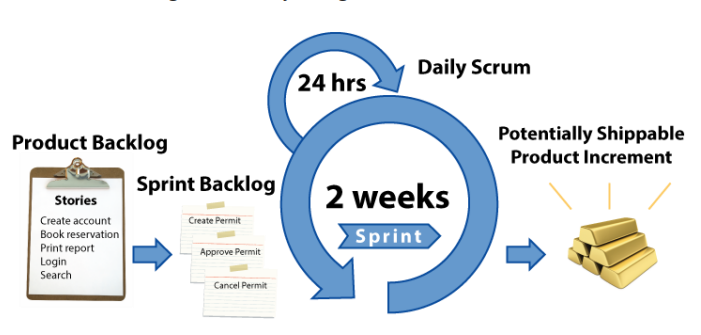
\includegraphics[keepaspectratio, width=12cm]{gambar/scrum-flow}
	\caption{Alur kerja scrum}
	\label{gambar:scrum-flow.png}
\end{figure}


\section{Perancangan \textit{User Interface}}

\textit{User Interface} adalah ilmu tentang tata letak grafis suatu web atau aplikasi \citep{userinterface1}. Cakupan \textit{User Interface} adalah tombol yang akan diklik oleh pengguna, teks, gambar, text entry fields, dan semua item yang berinteraksi dengan pengguna. Termasuk layout, animasi, transisi, dan semua interaksi kecil. UI mendesain semua elemen visual, bagaimana pengguna berinteraksi dengan halaman web dan apa yang ditampilkan di halaman web. Elemen visual yang ditangani oleh seorang desainer UI adalah skema warna, menentukan bentuk tombol, serta menentukan jenis font yang digunakan untuk teks. Desainer UI harus bisa membuat tampilan bagus yang akan meningkatkan kesetiaan pengguna. 
\subsection{Layout dan Spacing}
\textit{White spacing} merupakan jarak yang diberikan antara dua komponen baik itu jarak horizontal maupun vertikal. \textit{White spacing} diperlukan untuk memberikan setiap komponen ruang untuk bernafas. Dalam membuat \textit{white spacing} ada beberapa pendekatan diantaranya adalah pemberian \textit{white space} secara \textit{incremental} dari ukuran kecil hingga ke ukuran yang lebih besar. Pendekatan ini hanya meraih ukuran \textit{white spacing} minimum untuk terlihat bagus dan pada dasarnya dalam tampilan yang baik biasanya diperlukan lebih banyak white spacing. Pendeketan yang lebih baik dalam perancangan \textit{white spacing} yang baik adalah dengan mula mula memberikan komponen nilai \textit{white spacing} yang besar, dan lakukan pengurangan nilai \textit{white spacing} sampai pengguna merasa puas dengan nilai \textit{white spacing} yang diberikan. 

\begin{figure}[H]
	\centering
	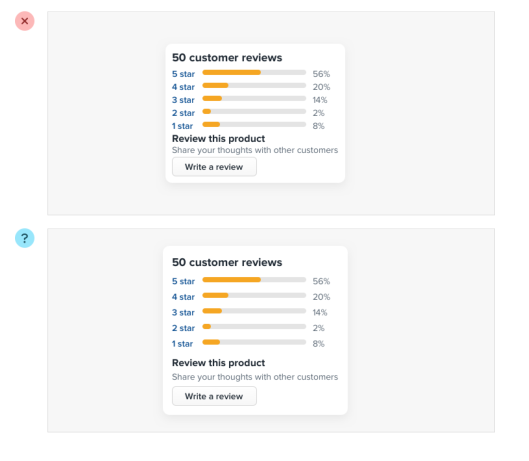
\includegraphics[keepaspectratio, width=12cm]{gambar/refactoring-ui-g1.png}
	\caption{Penentuan \textit{white spacing} dengan cara \textit{decremental} \citep{refactoringui}}
	\label{gambar:refactoring-ui-g1.png}
\end{figure}

Pada dasarnya komponen yang mempunyai banyak ruang untuk istirahat atau \textit{white spacing} terlihat lebih bersih dan simpel, namun ada beberapa kasus dimana \textit{white spacing} yang sedikit dan rapat dapat digunakan. Sebagai contoh, dalam perancangan tampilan \textit{dashboard}, yang dimana dalam tampilan \textit{dashboard} diperlukan untuk memuat informasi dalam jumlah banyak yang memungkinkan informasi tersebut terlihat dalam satu halaman.

\begin{figure}[H]
	\centering
	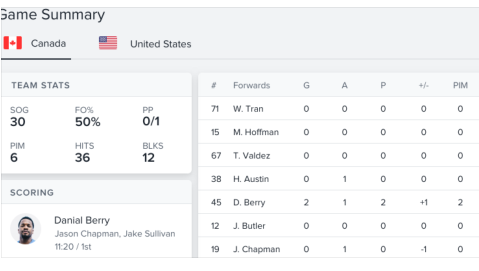
\includegraphics[keepaspectratio, width=12cm]{gambar/refactoring-ui-g2.png}
	\caption{Tampilan dashboard dengan nilai \emph{white spacing} yang kecil \citep{refactoringui}}
	\label{gambar:refactoring-ui-g2.png}
\end{figure}

Dalam mendesain sebuah \textit{layout} tidaklah harus mengisi seluruh \textit{white space} yang ada. Mengisi seluruh \textit{white space} yang ada hanya akan membuat tampilan lebih sulit untuk diinterpretasikan oleh pengguna.

\begin{figure}[H]
	\centering
	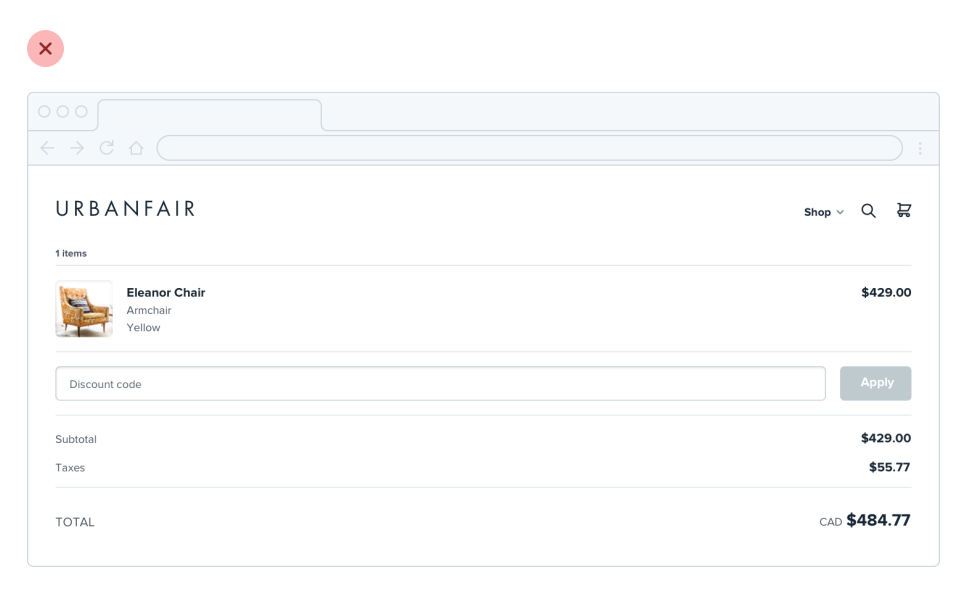
\includegraphics[keepaspectratio, width=12cm]{gambar/g-117.png}
	\caption{Komponen mengisi seluruh \textit{white space} dari sebuah halaman \citep{refactoringui}}
	\label{gambar:g-117.png}
\end{figure}

\begin{figure}[H]
	\centering
	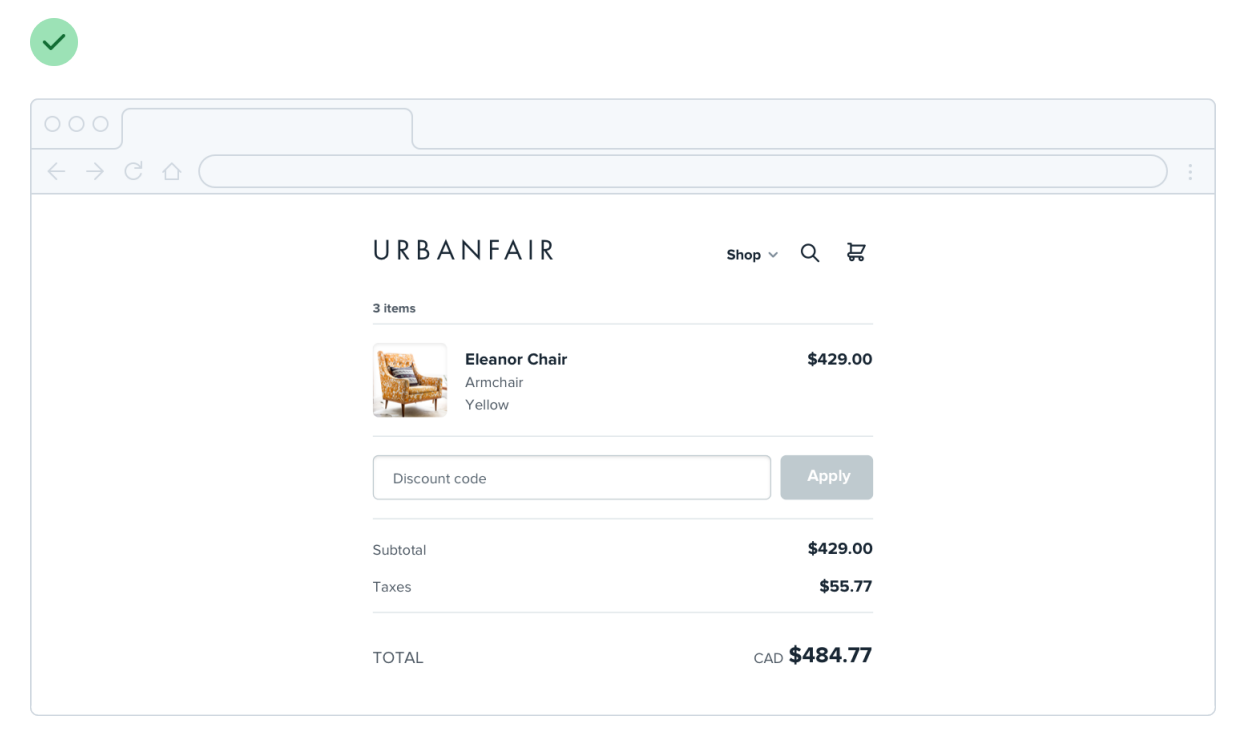
\includegraphics[keepaspectratio, width=14cm]{gambar/g-118.png}
	\caption{Komponen mengisi sebagian \textit{white space} dari sebuah halaman \citep{refactoringui}}
	\label{gambar:g-118.png}
\end{figure}

\subsubsection{Penentuan sistem desain \textit{spacing} dan \textit{sizing }}
%
%Dalam menentukan desain sistem untuk \textit{spacing} dan \textit{spacing} bukanlah hal yang mudah, dalam penentuannya tidaklah harus memilih-milih diantara dua ukuran atau lebih ukuran mana yang lebih baik atau lebih buruk, mencoba-coba beberapa ukuran untuk menemukan ukuran yang cocok adalah hal yang membuang waktu atau lebih parahnya lagi, membuat desain yang tidak konsisten. Pendekatan naif seperti memastikan ukuran \textit{spacing} dan \textit{sizing} dalam kelipatan 4 pixel tidaklah membantu permasalahan yang telah disebutkan. Dalam pembuatan sistem desain perlu diperhatikan hal seperti perbandingan relatif diantara dua nilai yang berdekatan. Contohnya adalah dalam skala kecil, penambahan beberapa \textit{pixel} dapat membuat perbedaan yang signifikan. Perubahan ukuran dari 12 \textit{pixel} ke 16 \textit{pixel} merupakan perubahan yang besar karena adanya 33 persen kenaikan.
%
%\begin{figure}[H]
%	\centering
%	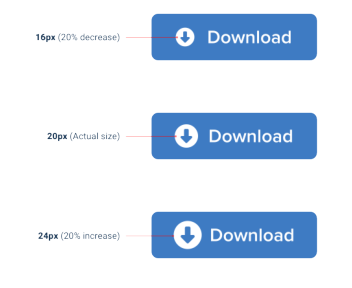
\includegraphics[keepaspectratio, width=12cm]{gambar/refactoring-ui-g4.png}
%	\caption{Perubahan pixel dalam skala kecil}
%	\label{gambar:refactoring-ui-g4.png}
%\end{figure}
%
%Akan tetapi dalam skala besar, perubahan beberapa \textit{pixel} adalah perubahan yang nyaris tidak terlihat, seperti perubahan ukuran dari 500 \textit{pixel} ke 520 \textit{pixel}, walaupun ada perbedaan 20 \textit{pixel} pada dua ukuran tersebut, perbedaan tersebut hanyalah 4 persen, 8 kali lipat kurang dari perubahan ukuran dari 12 \textit{pixel} ke 16 \textit{pixel}. Untuk mempermudah menentukan angka \textit{sizing} dan \textit{spacing}, pastikan saja ukuran diantara dua nilai tidak melebihi dari 25 persen. 
%
%\begin{figure}[H]
%	\centering
%	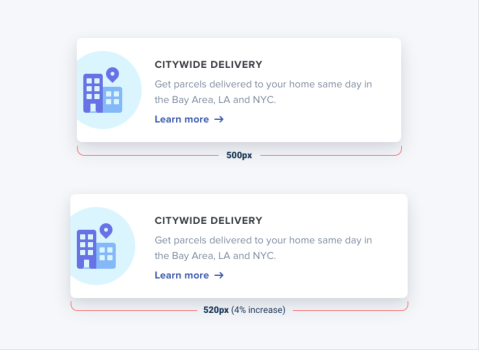
\includegraphics[keepaspectratio, width=12cm]{gambar/refactoring-ui-g3.png}
%	\caption{Perubahan pixel dalam skala besar}
%	\label{gambar:refactoring-ui-g3.png}
%\end{figure}

Dalam menentukan sebuah desain sistem ukuran \textit{sizing} dan \textit{spacing} tampilan, menghabiskan waktu dalam menentukan antara dua atau lebih nilai mana yang lebih baik untuk digunakan merupakan hal yang memakan waktu daripada menggunakan sistem yang telah ditentukan terlebih dahulu. Terdapat suatu pendekatan untuk menyelesaikan masalah tersebut dengan memulai dari menentukan nilai basis, dari nilai basis tersebut dapat dibuat rangkaian nilai skala dengan cara menggunakan nilai faktor dan mengalikannya dengan nilai basis yang telah ditentukan. Menggunakan nilai 16 \textit{pixel} sebagai basisnya disarankan dikarenakan 16 \textit{pixel} dapat dibagi secara baik dan merupakan setelan ukuran \textit{font browser} awal. Berikut ini merupakan contoh dari pendekatan yang telah disebutkan:

\begin{figure}[H]
	\centering
	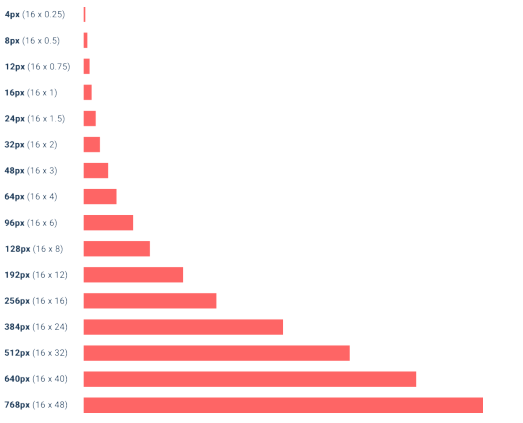
\includegraphics[keepaspectratio, width=8cm]{gambar/refactoring-ui-g5.png}
	\caption{Rangkaian nilai skala \citep{refactoringui}}
	\label{gambar:refactoring-ui-g5.png}
\end{figure}

\subsection{Text}
Kebanyakan tampilan yang ada menggunakan banyak sekali ukuran \textit{font}, bukan hal yang biasa untuk menemukan ukuran font dari ukuran 10 \textit{pixel} sampai 24 \textit{pixel} dalam satu tampilan. Hal ini merupakan hal yang tidak disarankan karena dua hal, desain yang tidak konsisten dan melambat pekerjaan.
\\
\begin{figure}[H]
	\centering
	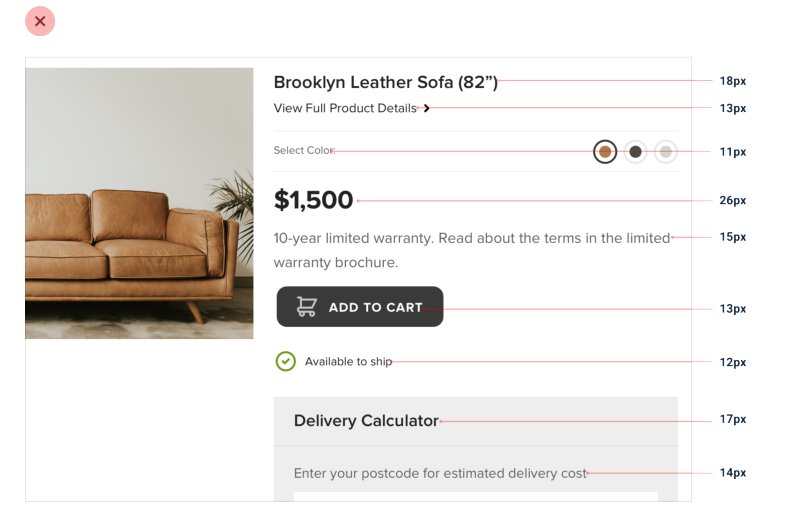
\includegraphics[keepaspectratio, width=8cm]{gambar/g100.png}
	\caption{Penggunaan ukuran font yang berlebihan dalam tampilan \citep{refactoringui}}
	\label{gambar:g100.png}
\end{figure}

%Dalam mendesain sistem desain untuk \textit{font}, sama seperti menentukan sistem desain {spacing dan sizing}, skala linear tidak dapat digunakan. 
Dalam membuat sistem desain font ada dua cara yaitu dengan menggunakan skala modular dan skala buatan sendiri.

Dalam skala modular, digunakan rasio seperti 4:5 ("\emph{a major third}"), 2:3 ("\emph{perfect fifth}") dan 1:1.618 ("\emph{golden ration}"). Dimulai dari menentukan nilai basis, mengaplikasikan rasio untuk mendapatkan angka selanjutnya dan mengaplikasikan nilai rasio tersebut lagi untuk mendapatkan nilai selanjutnya dan seterusnya. Pendekatan ini tampaknya menjanjikan, tapi dalam praktiknya, metode ini tidaklah sempurna karena beberapa alasan:

\begin{enumerate}
	\item{Dengan menggunakan skala modular dalam menentukan desain sistem \textit{font}, ukuran skala akan berakhir menggunakan angka pecahan, seperti  31.25 \textit{pixel}, 39.063 \textit{pixel}, 48.828 \textit{pixel} dan lain lainnya. \textit{Browser} menangani \textit{subpixel} sedikit berbeda sehingga nilai pecahan untuk ukuran text sebaiknya dihindari}.
	\item {Dengan menggunakan metode ini, ukuran skala yang dihasilkan adalah seperti 12 \textit{pixel}, 16 \textit{pixel}, 21 \textit{pixel} dan 28 \textit{pixel}. Hal ini membuat pemilihan ukuran font mejadi terbatas, pada praktiknya biasanya dibutuhkan nilai antara 21 \textit{pixel} dan 28 \textit{pixel} atau nilai antara 12 \textit{pixel} dan 16 \textit{pixel}}.
\end{enumerate}

\begin{figure}[H]
	\centering
	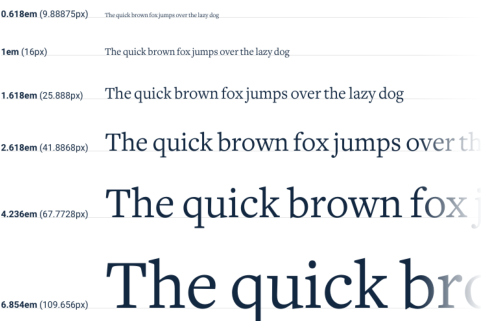
\includegraphics[keepaspectratio, width=12cm]{gambar/refactoring-ui-g6.png}
	\caption{Menentukan skala font menggunakan metode modular \citep{refactoringui}}
	\label{gambar:refactoring-ui-g6.png}
\end{figure}

Dalam skala buatan sendiri, penentuan nilai skala tidak dibatasi oleh formula matematika tetapi nilai skala ditentukan oleh pendesainnya sendiri. Dalam menggunakan metode ini tidak perlu lagi memerhatikan masalah seperti \textit{subpixel rounding} pada \textit{browser} dan juga dalam menggunakan metode ini, pendesain mempunyai kendali penuh dalam menentukan ukuran skala yang ada.

\begin{figure}[H]
	\centering
	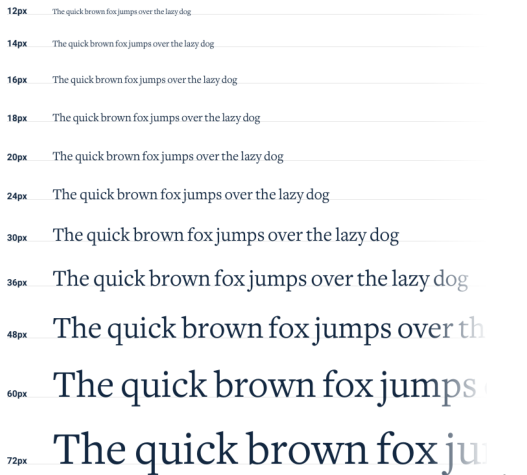
\includegraphics[keepaspectratio, width=12cm]{gambar/refactoring-ui-g7.png}
	\caption{Skala metode buatan sendiri \citep{refactoringui}}
	\label{gambar:refactoring-ui-g7.png}
\end{figure}

Pemilihan font yang akan digunakan dari ribuan \textit{font} yang tersedia secara tepat adalah hal yang sangat memakan waktu, kemampuan untuk melihat dan menentukan \textit{font} yang baik adalah kemampuan yang tidak dapat didapatkan secara singkat. Ada beberapa cara cepat untuk menentukan \textit{font} yang baik guna mengurangi waktu yang diperlukan untuk mempercepat proses pemilihan \textit{font} yaitu. 

\begin{enumerate}
	\item Untuk desain tampilan, pilihan yang aman adalah menggunakan \textit{typeface sans-serif} seperti Helvetica. Jika ragu untuk menggunakan \textit{font} yang dipilih, \textit{font} bawaan dari perangkat pengguna adalah pilihan tepat. Penggunaan \textit{font} dari bawaan perangkat pengguna membuat pengguna lebih familiar dengan tampilan yang dibuat karena pengguna sudah terbiasa dengan \textit{font} yang digunakan di perangkat meraka.
	\item Biasanya, \textit{font} didesain untuk tujuan yang spesifik. \textit{Font} yang memiliki \textit{letter-spacing} yang lebih rapat dan huruf \textit{lowercase} yang lebih pendek (\textit{shorter x-height}) biasanya digunakan untuk \textit{headline}, \textit{font} ini tidak cocok untuk digunakan sebagai \textit{font} utama dari tampilan . Sementara untuk \textit{font} yang digunakan untuk ukuran kecil seperti \textit{body} biasanya mempunyai \textit{letter-spacing} yang lebih lebar dan \textit{lowercase} letter yang lebih tinggi (\textit{taller x-height}).
	\begin{figure}[H]
		{\centering
			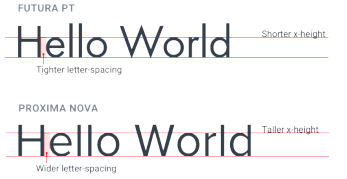
\includegraphics[keepaspectratio, width=12cm]{gambar/refactoring-ui-g9.png}
			\caption{Perbandingan \textit{font} untuk \textit{headline} dan \textit{body} \citep{refactoringui}}}
		\label{gambar:refactoring-ui-g9.png}
	\end{figure}
	\item Font yang populer kemungkinan besar adalah font yang bagus. Beberapa penyedia font di internet menyediakan fitur untuk mengurutkan font menurut urutan popularitas nya sehingga dapat mengurangi jumlah font yang harus dipilih.
	\begin{figure}[H]
		{\centering
			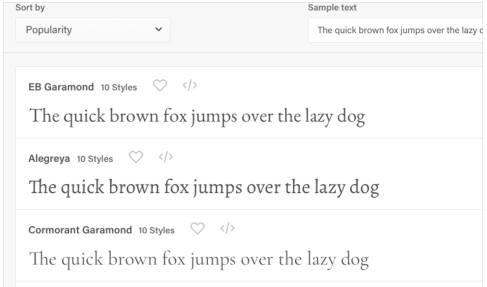
\includegraphics[keepaspectratio, width=12cm]{gambar/refactoring-ui-g10.png}
			\caption{Pengurutan berdasarkan popularitas \textit{font} \citep{refactoringui}}}
		\label{gambar:refactoring-ui-g10.png}
	\end{figure}
	\item Dimulai dengan mengunjungi beberapa situs favorit, biasanya dibalik situs tersebut, terdapat tim yang terdiri dari beberapa orang yang memiliki pengetahuan yang kuat tentang \textit{typography}. 
\end{enumerate}

Ketika mendesain paragraf, mudah sekali untuk membuat kesalahan dengan memuat seluruh teks ke dalam \textit{layout} yang ada dibandingkan dengan mencoba untuk membuat tampilan yang ramah untuk pembaca yang artinya teks akan terlihat sangat panjang dan sulit untuk dibaca.
\begin{figure}[H]
	{\centering
		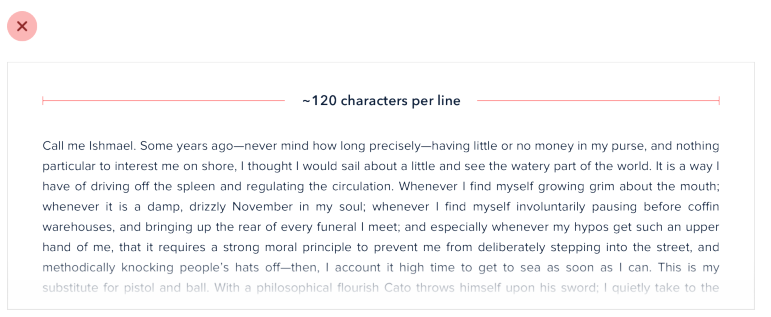
\includegraphics[keepaspectratio, width=16cm]{gambar/refactoring-ui-g11.png}
		\caption{Memuat banyak tulisan dalam sebuat \textit{layout} yang ada \citep{refactoringui}}}
	\label{gambar:refactoring-ui-g11.png}
\end{figure}

Untuk pengalaman membaca yang baik, paragraf haruslah dibuat untuk dapat menampung 45 sampai 75 karakter. Cara yang mudah dalam \textit{web} adalah menggunakan satuan unit \textit{em}, yang dimana satuan unit ini relatif dengan ukuran font \textit{web}. Ukuran yang tepat untuk ini adalah 20 \textit{em} sampai 35 \textit{em}.

\begin{figure}[H]
	{\centering
		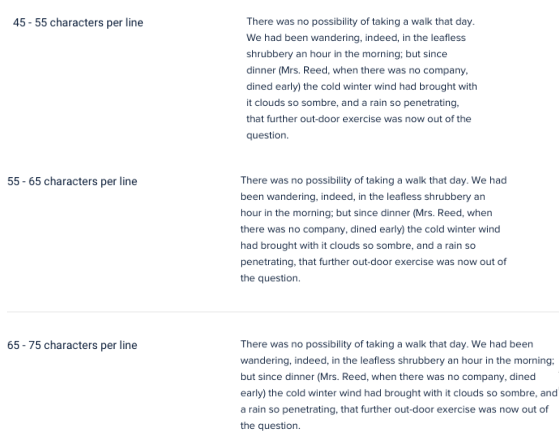
\includegraphics[keepaspectratio, width=14cm]{gambar/refactoring-ui-g12.png}
		\caption{Tampilan paragraf untuk ukuran 45-75 karakter \citep{refactoringui}}}
	\label{gambar:refactoring-ui-g12.png}
\end{figure}

Jika paragraf mengandung konten seperti gambar atau komponen yang besar, lebar text paragraf haruslah tetap dibatasi meskipun keseluruhan konten paragraf harus melebihi dari batas untuk menampung keseluruhan komponen.

\begin{figure}[H]
	{\centering
		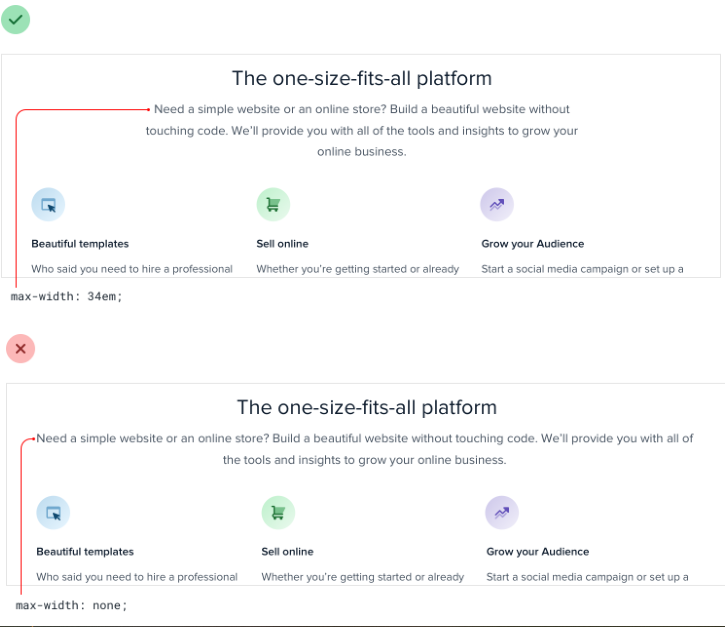
\includegraphics[keepaspectratio, width=12cm]{gambar/refactoring-ui-g13.png}
		\caption{Teks dengan komponen yang lebar dalam satu layout \citep{refactoringui}}}
	\label{gambar:refactoring-ui-g13.png}
\end{figure}

\subsubsection{\textit{Text Align}} 
Ada banyak situasi dimana diharuskan menggunakan beberapa ukuran \textit{font} dalam satu baris. Sebagai contoh dalam mendesain kartu dimana judul kartu tersebut memerlukan ukuran font yang lebih besar dibandingkan dengan elemen di sampingnya. Saat mencampur ukuran font seperti ini, biasanya secara insting, desainer akan cenderung melakukan \textit{center}-ing terhadap komponen tersebut untuk menciptakan keseimbangan.

 \begin{figure}[H]
	{\centering
		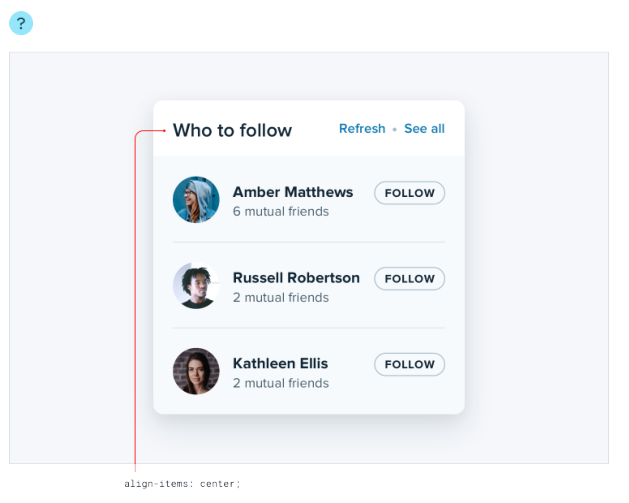
\includegraphics[keepaspectratio, width=10cm]{gambar/refactoring-ui-g14.png}
		\caption{Komponen kartu \citep{refactoringui}}}
	\label{gambar:refactoring-ui-g14.png}
\end{figure}

Ketika ada banyak ruang diantara dua komponen, hal ini terlihat baik baik saja. Namun jika kedua komponen teks tersebut didekatkan maka akan menjadi jelas bahwa tampilan akan terlihat buruk.
\begin{figure}[H]
	{\centering
		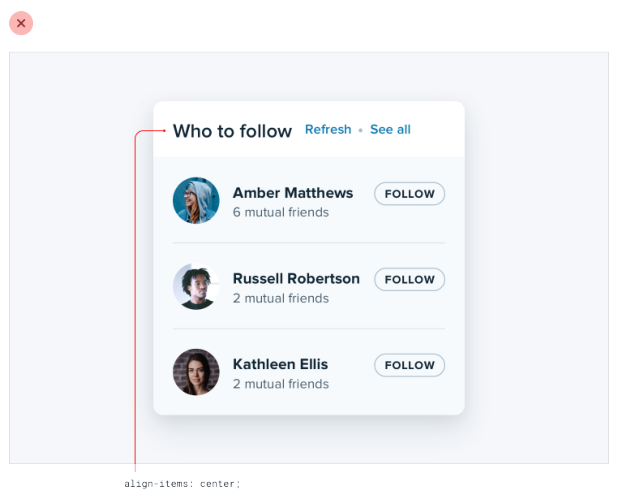
\includegraphics[keepaspectratio, width=10cm]{gambar/refactoring-ui-g17.png}
		\caption{Komponen kartu dengan komponen aksi dan judul didekatkan \citep{refactoringui}}}
	\label{gambar:refactoring-ui-g17.png}
\end{figure}

Pendekatan terbaik adalah menyelaraskan kedua komponen tersebut dengan \textit{baseline} atau sebuah garis imajinari tempat teks berdiri yang digunakan oleh teks untuk berdiri.
\begin{figure}[H]
	{\centering
		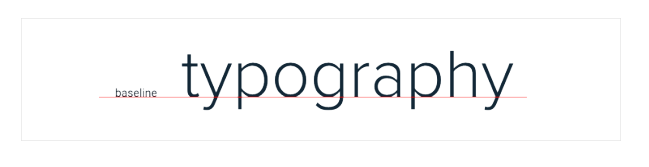
\includegraphics[keepaspectratio, width=12cm]{gambar/refactoring-ui-g18.png}
		\caption{\textit{Baseline} \citep{refactoringui}}}
	\label{gambar:refactoring-ui-g18.png}
\end{figure}
\begin{figure}[H]
	{\centering
		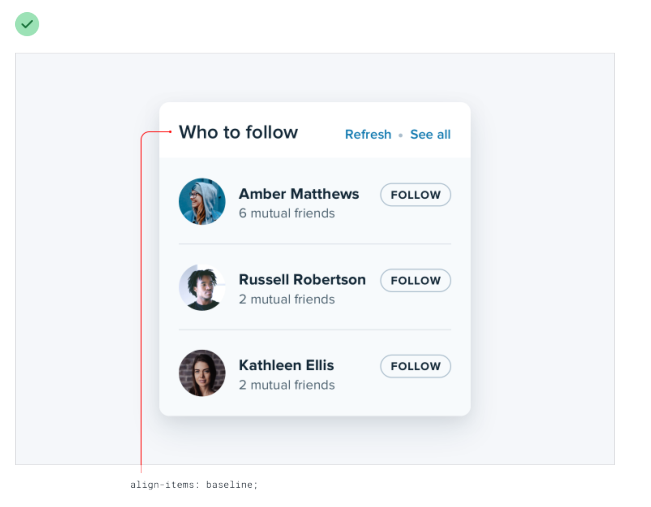
\includegraphics[keepaspectratio, width=12cm]{gambar/refactoring-ui-g19.png}
		\caption{Komponen aksi dan judul diselaraskan menurut \textit{baseline} \citep{refactoringui}}}
	\label{gambar:refactoring-ui-g19.png}
\end{figure}

\subsubsection{Letter spacing}
Pada umumnya ada baiknya untuk mempercayakan \textit{letter spacing} kepada pendesain \textit{font} tersebut. Namun ada beberapa kasus yang dimana mengubah \textit{letter spacing} dapat memperindah tampilan yang ada.
 \begin{figure}[H]
	{\centering
		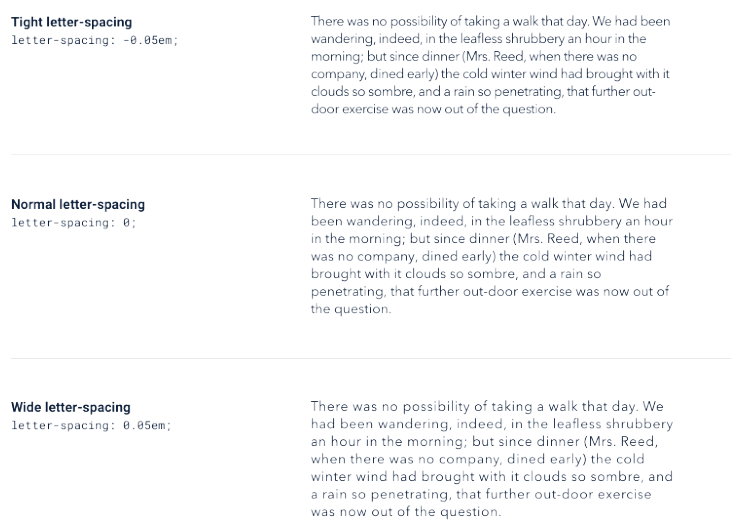
\includegraphics[keepaspectratio, width=12cm]{gambar/refactoring-ui-g21.png}
		\caption{\textit{Letter spacing} \citep{refactoringui}}}
	\label{gambar:refactoring-ui-g21.png}
\end{figure}
Ketika seseorang mendesain sebuah font, mereka mendesain \textit{font} tersebut dengan tujuan tertentu. \textit{Font family} seperti Open Sans didesain untuk keterbacaan dalam ukuran kecil yang dimana \textit{letter spacing} dari font family tersebut terlihat lebih besar dibandingkan dengan \textit{font family} seperti Oswald, yang dimana \textit{font family} Oswald digunakan untuk kebutuhan seperti penulisan judul utama.

\begin{figure}[H]
	{\centering
		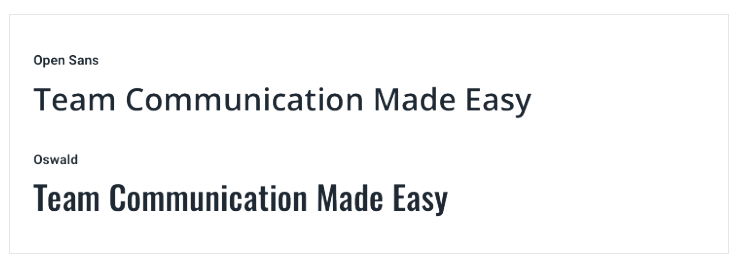
\includegraphics[keepaspectratio, width=12cm]{gambar/refactoring-ui-g22.png}
		\caption{\textit{Font family} Open Sans dan Oswald \citep{refactoringui}} }
	\label{gambar:refactoring-ui-g22.png}
\end{figure}

\textit{Font} yang dikhususkan untuk keterbacaan dalam ukuran kecil seperti Open Sans juga dapat digunakan untuk penulisan judul utama. Dengan mengurangi \textit{letter spacing} untuk meniru fungsi dari \textit{font family} seperti Oswald. Namun, hindari penggunaan sebaliknya, penggunaan \textit{font family} judul utama untuk keterbacaan dalam ukuran kecil memiliki kemungkinan kecil untuk bekerja.  

\begin{figure}[H]
	{\centering
		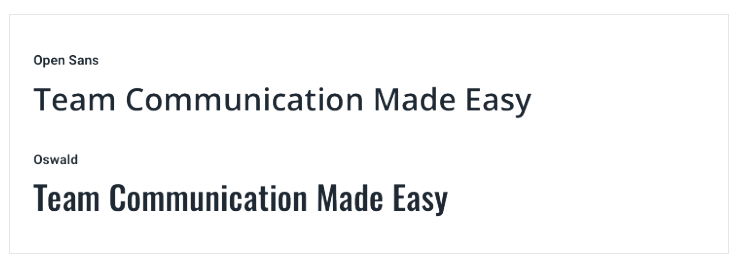
\includegraphics[keepaspectratio, width=12cm]{gambar/refactoring-ui-g22.png}
		\caption{\textit{Font family} Open Sans digunakan untuk \textit{headline} \citep{refactoringui}}}
	\label{gambar:refactoring-ui-g23.png}
\end{figure}

\subsection{Warna}
\subsubsection{\textit{Color Palette}}
\textit{Color palette} dapat dibagi menjadi tiga kelompok yaitu
\begin{enumerate}
	\item \emph{Abu abu} \hfill\\
	Warna yang biasanya terdapat pada beberapa komponen tampilan seperti \textit{form}, panel, warna latar belakang dan teks.
	\item \emph{Warna utama (\textit{primary color})} \hfill\\
	Warna yang digunakan dalam komponen seperti \textit{button}, navigasi dan lain lain. Warna ini mendefinisikan bagaimana suatu website terlihat, seperti contohnya ketika memikirkan sebuah merek seperti Facebook maka akan terpikirkan warna biru yang merupakan ciri khas dari Facebook sendiri.
	\item \emph{Warna aksen (\textit{accent color})} \hfill\\
	Warna aksen digunakan untuk menyampaikan maksud tertentu terhadap pengguna. Sebagai contoh, warna merah atau jingga digunakan untuk memikat pengguna terhadap fitur baru yang baru saja dirilis atau seperti warna merah yang digunakan untuk meminta konfirmasi pengguna untuk aksi yang destruktif.
	\begin{figure}[H]
		{\centering
			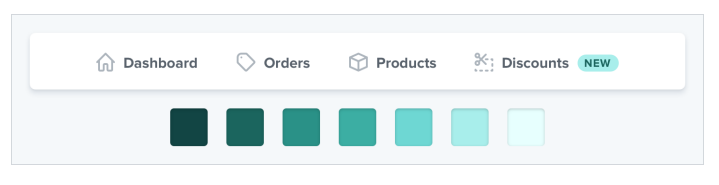
\includegraphics[keepaspectratio, width=12cm]{gambar/refactoring-ui-33.png}
			\caption{Penggunaan warna aksen untuk informasi \citep{refactoringui}}}
		\label{gambar:refactoring-ui-33.png}
	\end{figure}
	\begin{figure}[H]
		{\centering
			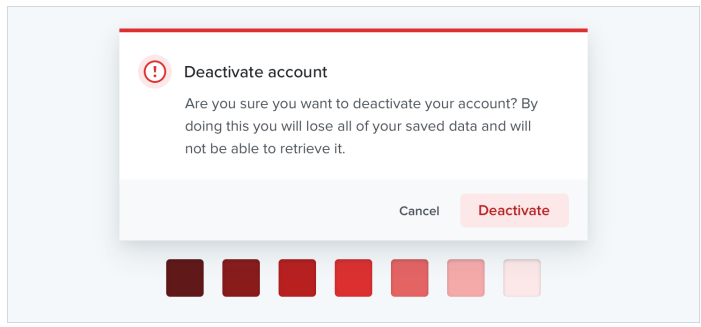
\includegraphics[keepaspectratio, width=12cm]{gambar/refactoring-ui-34.png}
			\caption{Penggunaan warna aksen untuk aksi destruktif \citep{refactoringui}}}
		\label{gambar:refactoring-ui-34.png}
	\end{figure}
\end{enumerate}

\subsubsection{Menentukan warna \textit{shade}} \textit{Shade} dapat ditentukan dari warna basis yang ada. Warna basis merupakan warna yang berada di tengah tengah antara shade yang paling gelap dan shade yang paling terang. Dalam penentuan basis warna sendiri, tidak ada formula khusus, melainkan terdapat beberapa cara yang dapat dipakai dalam menentukan basis warna. Caranya adalah mengambil basis warna shade yang cocok digunakan untuk warna \textit{background} dari elemen \textit{button}.
\begin{figure}[H]
	{\centering
		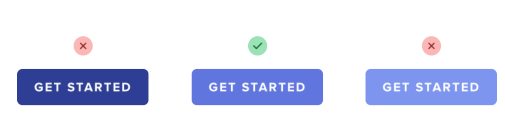
\includegraphics[keepaspectratio, width=12cm]{gambar/refactoring-ui-g40.png}
		\caption{Menentukan warna basis yang tepat menggunakan komponen \textit{button} \citep{refactoringui}}}
	\label{gambar:refactoring-ui-g40.png}
\end{figure}

Selanjutnya adalah menentukan sisi paling gelap dan sisi paling terang, dalam menentukan sisi yang paling gelap dan sisi yang paling terang dari warna shade tidak ada formula khusus yang dapat digunakan. Biasanya, sisi yang paling gelap digunakan untuk sebuah teks sedangkan sisi yang paling terang digunakan untuk sebuah \textit{background}. Dalam penentuannya dapat dimulai dengan menentukan basis warna lalu mengatur atribut \textit{saturation} dan \textit{lightness} hingga dirasa cocok.

\begin{figure}[H]
	{\centering
		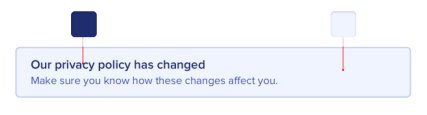
\includegraphics[keepaspectratio, width=12cm]{gambar/refactoring-ui-41.png}
		\caption{\textit{Shade} tergelap dan terterang \citep{refactoringui}}}
	\label{gambar:refactoring-ui-41.png}
\end{figure}

Saat selesai menentukan basis warna dan \textit{shade} warna paling gelap dan paling terang, langkah selanjutnya adalah mengisi ruang kosong yang ada. Pada umumnya, dibutuhkan sekurang kurangnya 5 warna \textit{shade} dalam suatu projek dan kurang lebih 10 warna \textit{shade} jika tidak ingin merasa dibatasi dengan pilihan warna. Angka 9 adalah angka yang tepat dikarenakan mudah untuk dibagi dan membuat mengisi ruang kosong yang ada lebih mudah. 900 adalah warna \textit{shade} paling gelap, 100 paling terang dan 500 adalah basis warna.

\begin{figure}[H]
	{\centering
		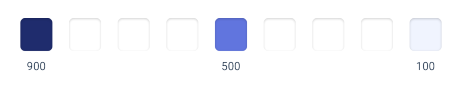
\includegraphics[keepaspectratio, width=12cm]{gambar/refactoring-ui-42.png}
		\caption{Nilai \textit{shade} untuk basis warna \citep{refactoringui}}}
	\label{gambar:refactoring-ui-42.png}
\end{figure}

Pengisian dimulai dari angka 700 dan 300 karena angka inilah yang berada di tengah tengah ruang kosong terus lanjutkan hingga semua ruang kosong terisi.

\begin{figure}[H]
	{\centering
		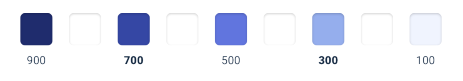
\includegraphics[keepaspectratio, width=12cm]{gambar/refactoring-ui-43.png}
		\caption{Pengisian nilai \textit{shade} untuk nilai 300 dan 700 \citep{refactoringui}}}
	\label{gambar:refactoring-ui-43.png}
\end{figure}

\begin{figure}[H]
	{\centering
		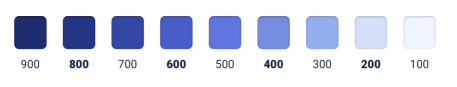
\includegraphics[keepaspectratio, width=12cm]{gambar/refactoring-ui-44.png}
		\caption{Pengisian nilai \textit{shade} untuk nilai 200, 400, 600 dan 700 \citep{refactoringui}}}
	\label{gambar:refactoring-ui-44.png}
\end{figure}

\subsubsection{\textit{HSL}} Hex dan RGB adalah dua format warna yang umum digunakan pada tampilan. Warna warna \textit{hex} dapat memiliki tampilan warna yang terlihat sama namun jika dilihat dari representasi kodenya, mereka terlihat tidak sama. HSL menyelesaikan masalah ini dengan mempresentasikan warna dengan atribut yang orang orang dapat merasakannya secara intuitif. Atribut yang dimaksud adalah \textit{hue}, \textit{saturation} dan \textit{lightness}.


\begin{figure}[H]
	{\centering
		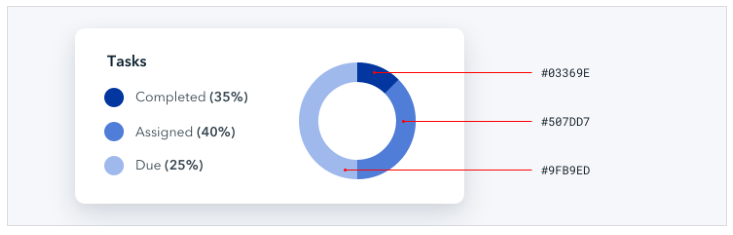
\includegraphics[keepaspectratio, width=12cm]{gambar/refactoring-ui-g24.png}
		\caption{Penggunaan \textit{hex} \citep{refactoringui}}}
	\label{gambar:refactoring-ui-g24.png}
\end{figure}

\begin{figure}[H]
	{\centering
		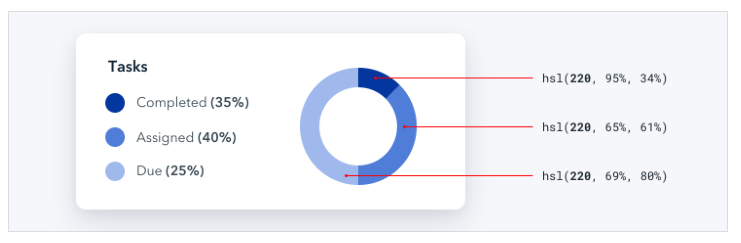
\includegraphics[keepaspectratio, width=12cm]{gambar/hsl-1.png}
		\caption{Penggunaan \textit{hsl} \citep{refactoringui}}}
	\label{gambar:hsl-1.png}
\end{figure}

\textit{Hue} merupakan atribut yang merupakan posisi warna di \textit{color wheel}. \textit{Hue} diukur dalam satuan derajat yang dimana 0 derajat melambangkan merah, 120 derajat melambangkan hijau dan 240 derajat melambangkan biru.
\begin{figure}[H]
	{\centering
		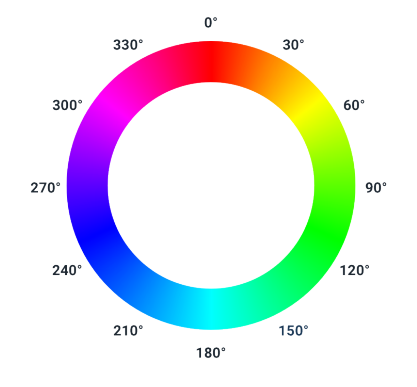
\includegraphics[keepaspectratio, width=12cm]{gambar/refactoring-ui-30png.png}
		\caption{\textit{Hue} \citep{refactoringui}}}
	\label{gambar:refactoring-ui-30png.png}
\end{figure}

\textit{Saturation} adalah nilai yang mengukur seberapa mencolok atau jelas suatu warna, 0\% \textit{saturation} menandakan warna abu abu (tidak ada warna),  sedangkan \textit{saturation} 100\% menandakan warna yang mencolok dan jelas. Tanpa \textit{saturation} nilai \textit{hue} tidaklah bermakna seberapapun nilainya karena warna akan tetap menjadi abu abu (tidak ada warna).
\begin{figure}[H]
	{\centering
		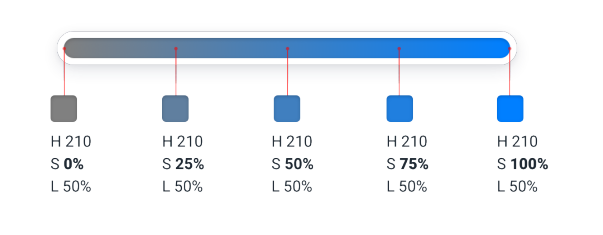
\includegraphics[keepaspectratio, width=12cm]{gambar/refactoring-ui-31.png}
		\caption{\textit{Saturation} \citep{refactoringui}}}
	\label{gambar:refactoring-ui-31.png}
\end{figure}

Atribut \textit{lightness} merupakan nilai yang mengukur seberapa dekat atau jauhnya sebuah warna dengan warna hitam maupun putih. 0\% \textit{lightness} adalah warna hitam, 100\% \textit{lightness} merupakan warna putih dan 50\% \textit{lightness} merupakan warna asli dalam nilai \textit{hue} tersebut.

\begin{figure}[H]
	{\centering
		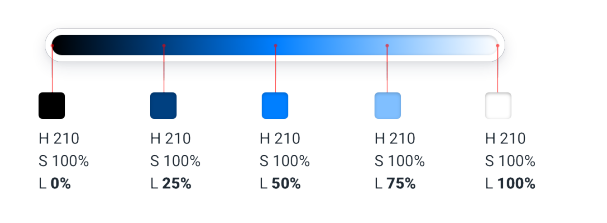
\includegraphics[keepaspectratio, width=12cm]{gambar/refactoring-ui-32.png}
		\caption{\textit{Lightness} \citep{refactoringui}}}
	\label{gambar:refactoring-ui-32.png}
\end{figure}

\subsubsection{\textit{Accessibility}}
Untuk mendesain tampilan yang \textit{accessible}, \textit{Web Content Accessibility Guidelines (WCAG)} merekomendasikan teks normal yang memiliki ukuran dibawah 18 \textit{pixel} memiliki kontras dengan perbandingan 4.5:1 dan teks yang lebih besar dari tersebut memiliki kontras tampilan setidaknya 3:1 untuk mendapat nilai kontras minimum (AA) dan kontras 7:1 untuk teks normal dibawah 18 dan 4.5:1 untuk teks yang lebih besar untuk mendapatkan nilai kontras yang tinggi (AAA).
\begin{figure}[H]
	{\centering
		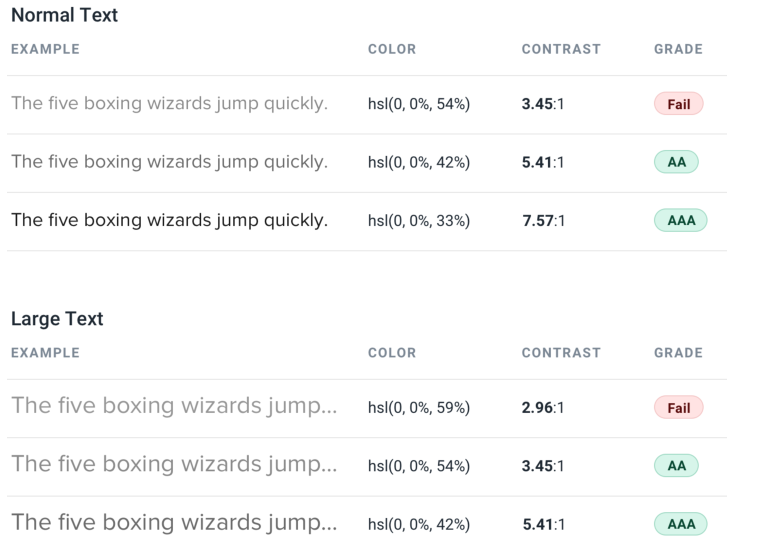
\includegraphics[keepaspectratio, width=12cm]{gambar/g-101.png}
		\caption{Kontras untuk teks ukuran normal dan besar \citep{refactoringui}}}
	\label{gambar:g-101.png}
\end{figure}

Untuk keperluan teks hitam diatas latar belakang yang cerah, memenuhi persyaratan perbandingan kontras yang direkomendasikan merupakan hal yang mudah. Namun, untuk memenuhi persyaratan yang direkomendasikan akan terasa sulit jika menggunakan warna. Ketika menggunakan teks putih diatas tampilan bewwarna diperlukan warna yang lebih gelap untuk memenuhi persyaratan kontras 4.5:1. 

\begin{figure}[H]
	{\centering
		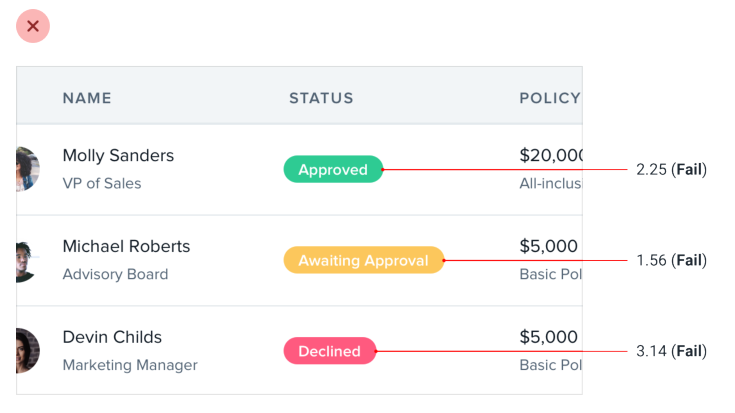
\includegraphics[keepaspectratio, width=12cm]{gambar/g-102.png}
		\caption{Teks putih diatas tampilan berwarna \citep{refactoringui}}}
	\label{gambar:g-102.png}
\end{figure}

Penambahan kegelapan warna dapat menimbulkan masalah hierarki kepada elemen yang seharusnya tidak menjadi fokus utama dari halaman. Latar belakang berwarna yang gelap akan mencuri perhatian pengguna.

\begin{figure}[H]
	{\centering
		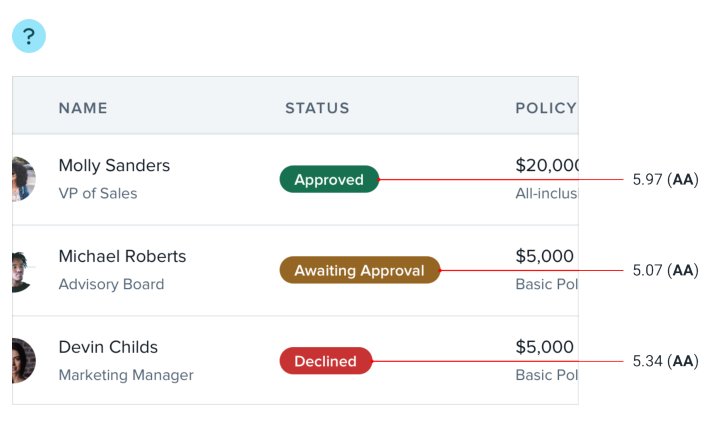
\includegraphics[keepaspectratio, width=12cm]{gambar/g-103.png}
		\caption{Tampilan warna yang gelap dapat mencuri perhatian pengguna \citep{refactoringui}}}
	\label{gambar:g-103.png}
\end{figure}

Permasalahan ini dapat diatasi dengan membalikan kontras. Daripada menggunakan teks dengan warna terang pada latar belakan berwarna gelap, menggunakan teks dengan warna gelap diatas latar belakang berwarna cerah merupakan pilihan yang tepat.

\begin{figure}[H]
	{\centering
		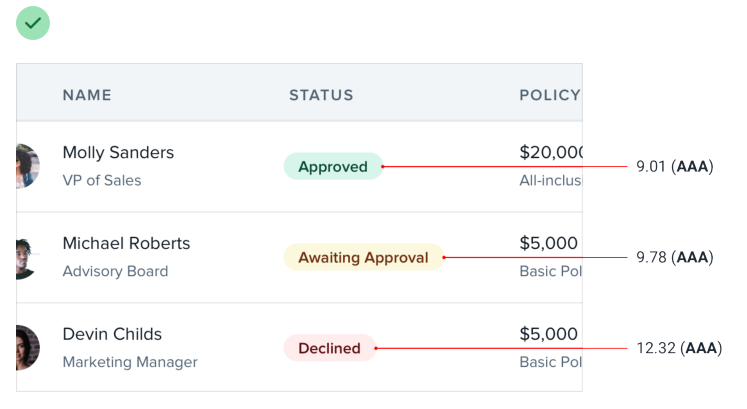
\includegraphics[keepaspectratio, width=8cm]{gambar/g-104.png}
		\caption{Pembalikan kontras antara teks dengan latar belakang \citep{refactoringui}}}
	\label{gambar:g-104.png}
\end{figure}

Untuk menyampaikan informasi kepada pengguna, warna saja tidaklah cukup dalam menyampaikan pengguna atau tidak pengguna dengan penyakit buta warna akan merasa kesulitan dalam menginterpretasikan tampilan yang ada. Sebagai contoh dalam gambar statistik di bawah ini, pengguna dengan buta warna hijau akan memiliki kesulitan dalam menentukan apakah statistik tersebut membaik atau memburuk.

\begin{figure}[H]
	{\centering
		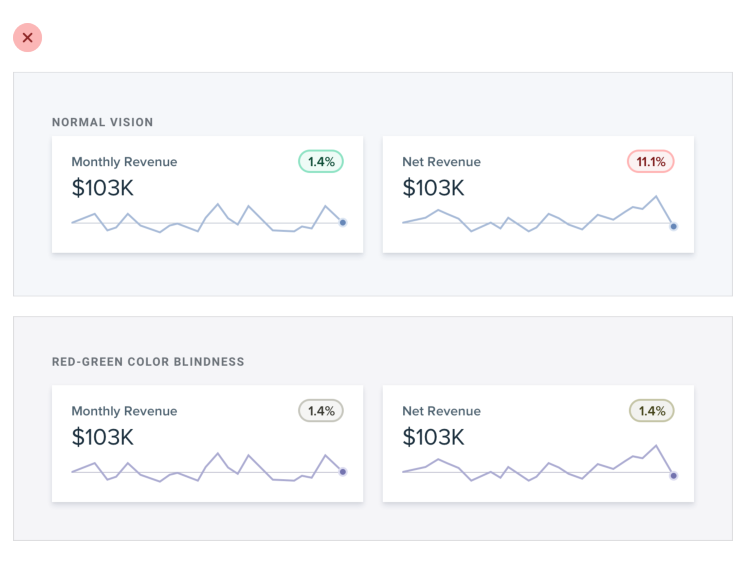
\includegraphics[keepaspectratio, width=8cm]{gambar/g-105.png}
		\caption{Warna saja tidak cukup dalam menyampaikan informasi \citep{refactoringui}}}
	\label{gambar:g-105.png}
\end{figure}

Untuk mengatasi masalah ini adalah dengan menambahkan cara lain untuk menyampaikan maksud kepada user, seperti menambahkan ikon yang mengindisakan perubahan positif atau negatif.

\begin{figure}[H]
	{\centering
		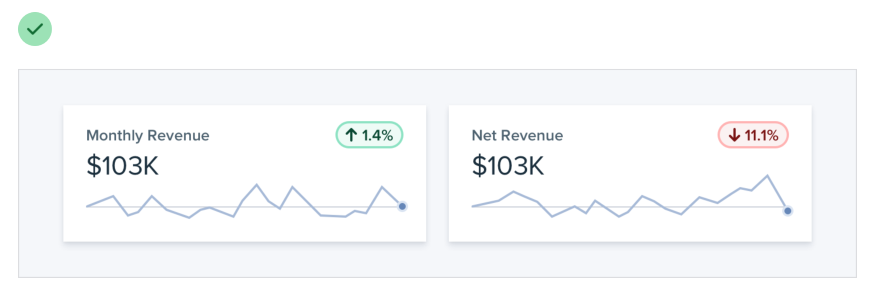
\includegraphics[keepaspectratio, width=12cm]{gambar/g-106.png}
		\caption{Penambahan ikon disamping warna untuk menyampaikan informasi \citep{refactoringui}}}
	\label{gambar:g-106.png}
\end{figure}

Untuk tampilan grafik yang terkadang memiliki banyak warna yang berbeda untuk setiap \textit{trend line}, akan lebih baik menggunakan perbedaan kontras daripada mengandalkan warna yang berbeda untuk setiap \textit{trend line}. Pengguna buta warna akan lebih mudah untuk mengenali perbedaan terang dan gelap dibandingkan dengan membedakan dua warna yang berbeda.
\begin{figure}[H]
	{\centering
		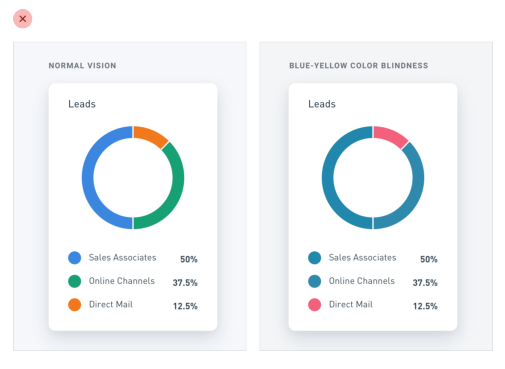
\includegraphics[keepaspectratio, width=10cm]{gambar/g-107.png}
		\caption{Menggunakan warna berbeda untuk setiap \textit{trend line} \citep{refactoringui}}}
	\label{gambar:g-107.png}
\end{figure}
\begin{figure}[H]
	{\centering
		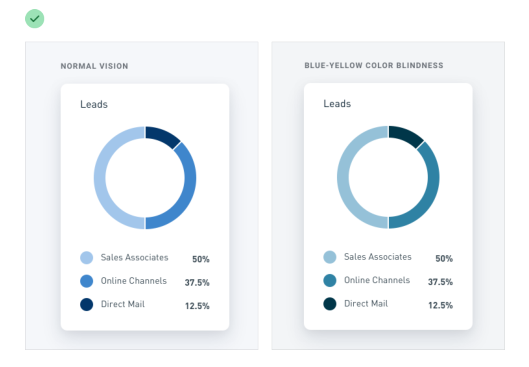
\includegraphics[keepaspectratio, width=10cm]{gambar/g-108.png}
		\caption{Menggunakan kontras yang berbeda untuk setiap \textit{trend line} \citep{refactoringui}}}
	\label{gambar:g-168.png}
\end{figure}


\section{Javascript}
\textit{Javascript} merupakan bahasa pemrograman tingkat tinggi dan bahasa pemrograman \textit{interpreted} yang biasanya digunakan untuk menambahkan interaktivitas dan sifat dinamis dalam sebuah \textit{websites}. Javascript biasa dikenal sebagai "Bahasa \textit{Web}" dikarenakan javascript didukung oleh mayoritas \textit{web browsers} dan dapat membuat elemen yang interaktif, memanipulasi konten sebuah \textit{website} dan merespon aksi pengguna.

Javascript di kembangkan oleh Brendan Eich pada tahun 1995 ketika Brendan Eich sedang bekerja pada perusahaan Netscape Communications Corporation. Pengembangan javascript dilakukan karena adanya kebutuhan bahasa \textit{scripting} yang dapat menambahkan interaksi dan fungsi dinamis dalam \textit{website}. Pada saat itu, kebanyakan \textit{website} merupakan statis dan kekurangan kemampuan dalam merespon interaksi pengguna.

Sebelummnya bernama "Mocha", bahasa ini kemudian berganti nama menjadi "Livescript" dan pada akhirnya "Javascript" untuk kebutuhan marketing, memanfaatkan popularitas bahasa pemrograman Java pada saat itu. Meskipun Javascript dan Java memiliki nama yang hampir mirip, keduanya merupakan bahsa yang berbeda dengan prinsip desain dan tujuan yang berbeda.

Seiring berkembangnya popularitas javascript, \textit{web browser} lainnya seperti Microsoft dengan Internet Explorer dan Mozilla dengan Firefox, mengimplementasikan dukungan untuk bahasa pemgrograman javascript. Adopsi javascript ke dalam \textit{web browser} terkenal tersebut membuat pendukung yang kuat bagi javascript untuk menjadi stndar \textit{de facto} untuk \textit{client-side scripting} pada \textit{website}.

Selama bertahun tahun, Javascript telah mengalami perubahan yang signifikan dengan adanya fitur-fitur baru, improvisasi dan penambahan pada bahasa Javascript. AJAX atau \textit{Asynchronous Javascript and XML} pada awal tahun 2000 mengembangkan kemampuan Javascript lebih jauh lagi dengan kemampuannya melakukan komunikasi \textit{asynchronous} dengan \textit{server} melakukan perubahan data yang dinamis pada halaman \textit{website} tanpa melakukan muat ulang halaman \textit{website}.

Dalam akhir akhir ini, Javascript telah berkembang melebihi dari kebutuhan aslinya. Dengan pengenalan NodeJS, program yang dapat menjalankan Javascript di luar browser. Dengan ini, Javascript dapat digunakan dalam berbagai bidang seperti \textit{server-side scripting}, \textit{command-line tools} dan membuat aplikasi. Javascript juga telah tumbuh lebih signifikan lagi dengan perkenalan berbagai \textit{framework}, \textit{library} dan \textit{tools} yang mensimplifikasikan proses pengembangan. \textit{Framework} popular sperti Angular, React dan VueJS telah diadopsi oleh banyak orang, memberikan pengembang alat untuk membuat aplikasi \textit{web} yang kompleks.

\section{Three JS}
Three.js merupakan sebuah library dari Javascript untuk
membuat dan menampilkan grafik 3D pada web browser. Dengan menggunakan Three JS, pembuatan tampilan 3 dimensi lebih mudah untuk dilakukan dikarenakan Three JS sudah menyediakan beberapa fitur seperti \textit{scenes}, \textit{camera}, \textit{lights}, \textit{shadows}, \textit{materials}, \textit{textures}, \textit{3d math} dan lain lain.
\subsection{\emph{Camera}}
\textit{Camera} mendefinisikan bagaimana apa yang akan kita lihat jika kita me-\textit{render} \textit{scene}. Jenis \textit{camera} yang paling banyak digunakan dalam three js adalah \textit{perspective camera} yang memberikan efek 3d dimana objek dekat terlihat lebih besar sedangkan objek yang letaknya jauh terlihat lebih kecil.
\textit{Perspective camera} mendefinisikan fructumnya melalui empat properties yaitu \textit{near} yang mendefinisikan dimana letak frustum depan, \textit{end} mendifinisikan dimana itu berakhir, \textit{fov} atau \textit{field of view} merupakan bagian dari scene yang dapat terlihat dari \textit{camera} dan \textit{aspect} merupakan perbandingan antara garis vertikal dan horizontal dari \textit{scene} yang akan ditampilkan.

\begin{figure}[H]
	\centering
	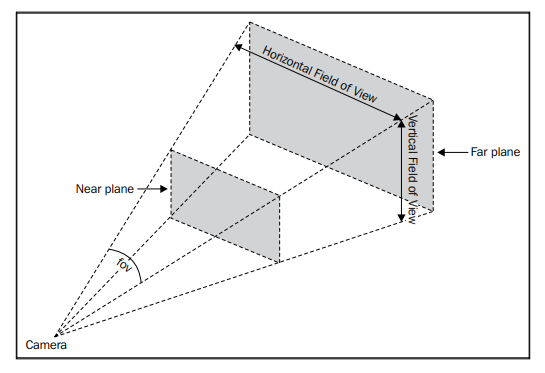
\includegraphics[keepaspectratio, width=12cm]{gambar/fructum}
	\caption{Frustum Camera ThreeJS}
	\label{gambar:fructum.png}
\end{figure}

\subsection{\emph{Mesh}}
Mesh merupakan objek triangular polygon yang dibuat dengan gabungan antara objek Geometry dan  Material. Mesg juga merupakan basis objek dari berbagai objek mesh lainnya seperti Skinned Mesh, MorhAnimMesh dan lain lain.
\begin{figure}[H]
	\centering
	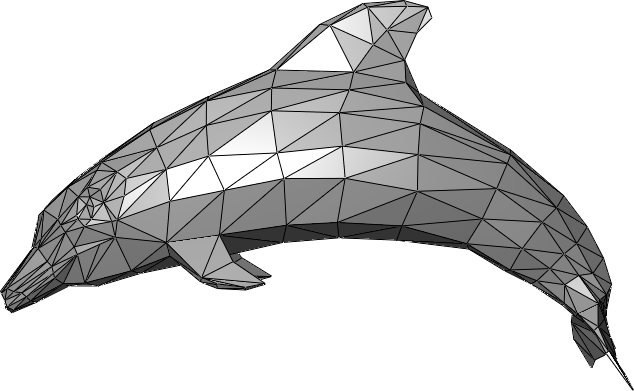
\includegraphics[keepaspectratio, width=8cm]{gambar/mesh.png}
	\caption{Mesh ThreeJS}
	\label{gambar:mesh.png}
\end{figure}

\subsection{\emph{Scene Graph}}
\textit{Scene graph} merupakan struktur seperti pohon yang terdiri dari beberapa objek seperti \textit{scene}, \textit{camera}, \textit{mesh} dan lain lain. Objek objek tersebut berstruktur secara hierarki dengan hubungan seperti \textit{parent} dan \textit{child} dan merepresentasikan dimana objek akan muncul dan bagaimana mereka berorientasi. \textit{Children} diposisikan dan diorientasikan sesuai dengan \textit{parent} mereka. 

\begin{figure}[H]
	\centering
	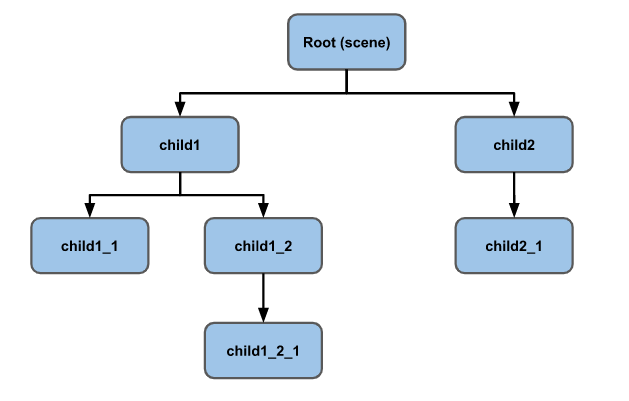
\includegraphics[keepaspectratio, width=12cm]{gambar/tree-graph-three}
	\caption{Scene Graph ThreeJS}
	\label{gambar:tree-graph-three.png}
\end{figure}

\subsection{\emph{Primitives}}
\textit{primitives} merupakan bentuk 3-dimensi yang dihasilkan saat program berjalan dengan beberapa parameter yang telah ditentukan. Three JS memiliki beberapa \textit{primitives} bawaan seperti \textit{BoxGeometry}, \textit{CircleGeometry}, \textit{CylinderGeometry}, \textit{ConeGeometry} dan lain lain dengan parameter yang dapat ditentukan untuk setiap masing masing bentuk sesuai dengan keinginan. 

\begin{figure}[H]
	\centering
	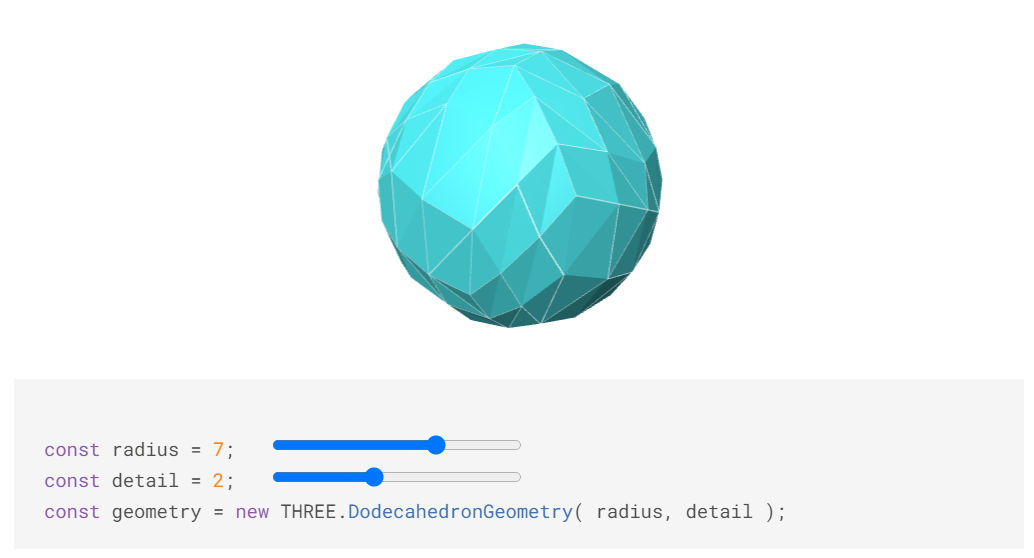
\includegraphics[keepaspectratio, width=12cm]{gambar/three-js-geometry-example.png}
	\caption{Primitives ThreeJS}
	\label{gambar:three-js-geometry-example.png}
\end{figure}

\subsection{\emph{Drag Controls}}
Pustaka ThreeJS menyediakan berbagai macam \textit{control}, salah satunya adalah \textit{Drag Controls}. Drag Controls memungkinkan pengguna menggunakan fitur \textit{drag and drop} untuk tampilan objek tiga dimensi pada tampilan. \textit{Drag Controls} tidak termasuk dalam fungsi yang disediakan secara langsung oleh ThreeJS melainkan fitur \textit{Drag Controls} ini tersedia bagi user dalam sebuah addon yang harus di-\textit{import} secara manual oleh pengguna.


\section{\textit{Unit Testing}}

%Pengujian perangkat lunak merupakan sesuatu yang penting untuk memastikan perangkat lunak yang dibuat dapat berjalan sesuai dengan fungsionalitas yang diharapkan. Pengujian sendiri merupakan elemen penting untuk memastikan kualitas perangkat lunak yang baik dan merupakan bagian yang tidak dapat dipisahkan dari siklus hidup pengembangan perangkat lunak seperti halnya analisis, desain, dan pengkodean \citep{ut1}.

\textit{Unit testing} merupakan salah satu teknik yang biasa digunakan untuk melakukan pengujian perangkat lunak yang berfokus pada bagian terkecil dari sebuah aplikasi. \textit{Unit testing} memungkinkan untuk menguji perangkat lunak secara terpisah dengan menguji bagian unit terkecil dan beberapa potongan kode seperti fungsionalitas perangkat lunak. Cara yang biasa dilakukan untuk \textit{unit testing} adalah menulis kode \textit{unit testing} dan \textit{test case} secara manual ketika akan melakukan pengujian. Pengujian unit fokus pada usaha verifikasi pada unit yang terkecil pada desain perangkat lunak (komponen atau modul perangkat lunak). Setiap unit perangkat lunak diuji agar dapat diperiksa apakah aliran masukan (\textit{input}) dan keluaran (\textit{output}) dari unit sudah sesuai dengan yang diinginkan. Pengujian unit biasanya dilakukan saat kode program dibuat \citep{ut2}.

\section{\textit{User Acceptance Testing}}
%
%\textit{User Acceptance Testing} merupakan pengujian yang dilakukan oleh \textit{end-user} dimana \textit{user} tersebut adalah staff/karyawan perusahaan yang langsung berinteraksi dengan sistem dan dilakukan verifikasi apakah fungsi yang ada telah berjalan sesuai dengan kebutuhan/fungsinya. Setelah dilakukan sistem testing, \textit{user acceptance testing} menyatakan bahwa sistem perangkat lunak memenuhi persyaratan \citep{uat1}. Kegiatan \textit{user acceptance testing} dapat dilakukan di ujung akhir pengerjaan suatu projek ataupun di akhir dari setiap iterasi pengerjaan yang dilakukan \citep{uat}.
%
%\textit{User Acceptance Test} memastikan bahwa aplikasi yang akan dibuat akan memenuhi harapan dari pengguna dan bekerja dengan baik sesuai dengan apa yang diharapkan oleh pengguna. Dapat disimpulkan bahwa \textit{user acceptance testing} adalah pengujian yang dilakukan oleh \textit{user} atau pengguna yang dimana adalah staff/karyawan dari sebuah sistem untuk memastikan fungsi-fungsi yang ada pada sistem yang telah dibuat tersebut telah berjalan dengan baik dan sesuai dengan kebutuhan pengguna.


\textit{User Acceptance Testing} merupakan pengujian yang dilakukan oleh \textit{end-user} dimana \textit{user} tersebut adalah staff/karyawan perusahaan yang langsung berinteraksi dengan sistem dan dilakukan verifikasi apakah fungsi yang ada telah berjalan sesuai dengan kebutuhan/fungsinya. Setelah dilakukan sistem testing, \textit{user acceptance testing} menyatakan bahwa sistem perangkat lunak memenuhi persyaratan \citep{uat1}. Kegiatan \textit{user acceptance testing} dapat dilakukan di ujung akhir pengerjaan suatu projek ataupun di akhir dari setiap iterasi pengerjaan yang dilakukan \citep{uat}. Pada penelitian ini \textit{user acceptance testing} digunakan untuk memastikan bahwa aplikasi yang sudah dibuat sudah memenuhi kebutuhan pengguna atau tidak.

\section{Visualisasi Data}
Penggunaan kata visualisasi berasal dari latin yaitu "visualis" dan memiliki arti yaitu menggambarkan, obbservasi dan menyajikan hasil visual dari observasi dan analisis informasi digital atau suatu peristiwa. Visualisasi data merupakan proses menginterpretasi hasil analisisi dengan berbagai cara untuk mewujudkan pengambilan keputusan yang lebih efisien.

Tabel merupakan metode yang sudah lama digunakan untuk mengklasifikasikan, mengorganisir dan menyajikan informasi kuantitaif dan kualitatif. Salah satu tujuan penggunaan tabel adalah untuk menampilkan data kuantitatif dengan menunjukan hubungan simpel antara nilai kuantitatif dan kategori yang mana nilai ini terhubung sehingga nilai nilai tersebut dapat diletakan dan dihubungan secara sendiri sendiri. Tabel memungkinkan menampilkan data dalam jumlah banyak dalam ruang yang sedikit, membuat pembaca dapat melihat keseluruhan data yang banyak dengan cepat. Beberapa konsep basik dari desain tabel adalah \citep{datavisualization1}

\begin{enumerate}
	\item Hubungan ditampilkan dalam tabel dibagi menjadi dua yaitu: \textit{quantitative-to-categorical} digunakan untuk melihat satu data kuantitatif dalam satu waktu dan \textit{quantitative-to-quantitative} untuk memperlihatkan hubungan antara data data.
	\item Tabel dapat didesain dalam dua cara yaitu: (1) \textit{unidirection} yaitu dimana kategori dalam bentuk baris atau kolom, tidak dapat keduanya (2) \textit{bidirectional}, atau disebut multidirectional yang dimana lebih dari dua pasang kelompok kateogri.
	\item Semua teks dalam tabel haruslah disusun secara horizontal. Judul kolom harus diulang setiap ada kelompok baru dalam kasus dimana tabel melebihi dari satu halaman. \textit{Text alignment} dalam tabel numerikal haruslah konsisten untuk menunjukan data secara jelas.
\end{enumerate}

Grafik menerjemahkan data kedalam bentuk objek visual dan merupakan alat yang kuat untuk menyampaikan informasi kuatitatif. Grafik digunakan saat dimana ketika sulit untuk mempresentasikan pola, tren atau hubungna informasi dalam bentuk verbal atau dalam bentuk tabel. Ada beberapa type grafik yang biasanya digunakan, yaitu: \citep{datavisualization1}

\begin{enumerate}
	\item{Grafik Batang, menurut Bigwood dan Spore merupakan grafik dalam bentuk kolom dan batang yang disusun secara vertical maupun horizontal dan dirancang untuk mempresentasikan hubungan antara dua atau lebih pasangan data.}
	\item{Garif garis, menurut Few mempresentasikan informasi berupa garis dan sangat cocok untuk memvisualisasikan bagaimana nilai data berubah setiap waktu, menampilkan kontinuitas, alur dan fluktuasi nilai}
	\item{Grafik pie didesain untuk memvisualisasikan proporsi atau sebagian dari keseluruhan}
\end{enumerate}

Dalam pembuatan grafik ini, ada beberapa elemen desain grafik atau dapat disebut \textit{non-data elements}, biasanya elemen desain ini dipergunakan untuk memperhidup tampilan grafik, kebutuhan artistik, sebagai dekorasi dan lain lain. jika tidak diperhatikan dengan baik, penggunaan berlebihan elemen non data ini bisa berujung menjadi "\textit{chartjunk}". Berikut ini adalah beberapa prinsip penting dalam perencanaan dan pendesainan grafik: \citep{datavisualization1}
\begin{enumerate}
	\item {Elemen grafik seperti \textit{axis} dan \textit{grids} bertujuan sebagai struktur pendukung dan mendefinisikan dimana data harus ditampilkan. Oleh karenanya komponen ini tidaklah harus dibuat mencolok mengalihkan perhatian dari data, elemen ini seharusnya hanya ditampilkan seminimal mungkin untuk melakukan fungsinya saja.}
	\item{\textit{Fills atau pattern} haruslah dipilih secara hati hati, karena hal ini jika tidak dipilih secara hati hati dapat mengakibatkan distraksi atau misinterpretasi data yang disajikan. Penggunaan elemen seperti (\textit{stripes}, \textit{weaves}, \textit{checkers}, \textit{dots}) membuat ilusi yang dapat disebut \textit{fabric effect} }
	\item {Perhatian khusus harus diberikan kepada pemberian efek tiga dimensi untuk mempresentasikan data yang dimana penggunaan efek ini menjadi luas karena fitur ini disediakan oleh perangkat lunak \textit{spreadsheet} konvensional yang beredar di pasaran. Kebanyak peneliti setuju bahwa penggunaan efek ini haruslah dihindari.}
	\item {Menurut Bigwood dan Spore, Pelabelan data yang sesuai juga memainkan peran penting dalam mempresentasikan data secara grafikal dan aspek seperti jarak antara elemen grafik, orientasi horizontal teks, dan pengunaan kalimat yang jelas juga penting dalam menyajikan informasi yang akurat. Penggunaan legenda jugalah harus diperhatikan. Beberapa penulis berpendapat bahwa penggunaan legenda sebaiknya digunakan ketika kasus dimana label data terlalu panjang untuk dimuat dalam elemen grafik. Beberapa penulis juga setuju peletakan komponen legenda ini haruslah sedekat mungkin dengan grafik. }
\end{enumerate}


\section{Participatory Design}
\textit{Participatory design} merupakan suatu kumpulan teori, praktis dan ajaran yang mengikut sertakan dengan pengguna dalam aktivitas yang mengarah ke produk perangkat lunak dan perangkat keras \citep{participatory}. Banyak peneliti dan praktisi dalam \textit{Participatory design} termotivasi dalam improvisasi proses internal dan kombinasi dari berbagai pengetahuan untuk membuat pelayanan dan produk yang lebih baik.

\textit{Participatory design} bermula dari Scandinavia pada tahun 1970-an dan 1980-an. Karya Scandinavian ini dipicu oleh komitmen dari Marxist untuk memberdayakan pekerja dan membina demokrasi dalam tempat kerja. Persatuan buruh mempuyai pengalaman yang rendah mengenai teknologi komputer dan terpaksa diharuskan untuk menerima sistem yang dikembangkan oleh manajemen, sistem yang merepresentasikan ketidaksesuaian dengan cara kerja pekerja pada biasanya. Oleh karena mereka tidak mengerti dalam mendesain sebuah teknologi komputer mereka sendiri, para pekerja ditempatkan dalam posisi menerima atau menolak teknologi yang ada. Beberapa peneliti Scandinavia mengutarakan cara pengembangan, sebuah pendekatan yang menyajikan "\textit{language games}"

\textbf{}
%
%\section{Analisa Desain Database}
%
%Teknologi database yang digunakan untuk penelitian search engine \citep{lazu} adalah MySQL yang merupakan database SQL. Adapun relasi tabel tabel yang digunakan pada penelitian sebelumnya adalah sebagai berikut. 
%
%\begin{figure}[H]
%	{\centering
%		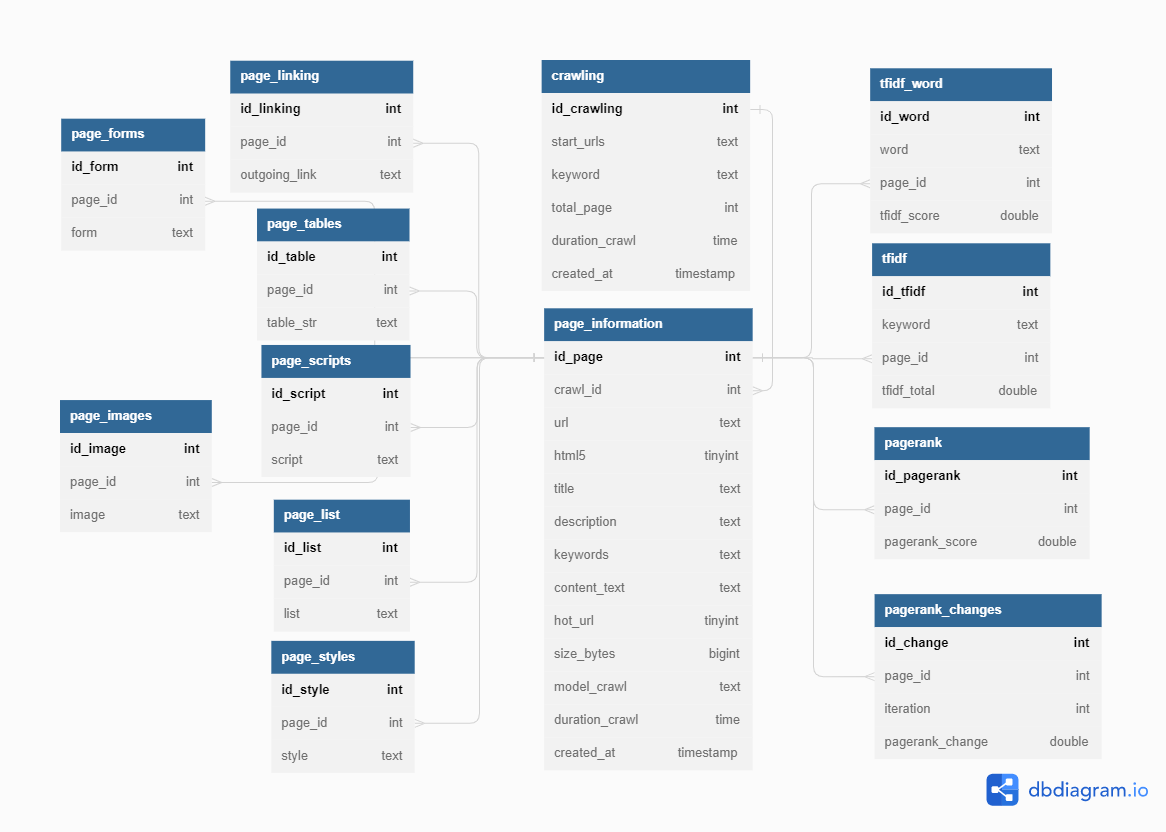
\includegraphics[keepaspectratio, width=12cm]{gambar/ERD Crawler.png}
%		\caption{Skema database yang digunakan dalam proses crawling}}
%	\label{gambar:ERD Crawler.png}
%\end{figure}
%
%Pada saat proses \textit{crawling} berjalan, \textit{crawler} membutuhkan beberapa tabel untuk menyimpan informasi yang didapatkan \textit{crawler} dalam proses berjalannya. Tabel-tabel tersebut diantaranya adalah: \textit{page linking} merupakan tabel untuk menyimpan link keluar dari suatu halaman, \textit{page images} digunakan untuk menyimpan semua gambar yang ada dalam suatu halaman, \textit{page scripts} digunakan untuk menyimpan semua \textit{script} yang terdapat dalam suatu halaman, \textit{page tables} digunakan untuk menyimpan semua tabel yang terdapat pada suatu halaman, \textit{page styles} digunakan untuk menyimpan \textit{style} yang bertugas untuk memberi tampilan pada suatu halaman, \textit{page forms} untuk menyimpan semua form yang terdapat dalam suatu halaman dan \textit{page list} untuk menyimpan seluruh \textit{list} dalam suatu halaman. Masing masing dari tabel yang telah disebutkan terbeut berhubungan \textit{Many to one} dengan tabel \textit{page information}. Sedangkan untuk tabel yang digunakan untuk \textit{document ranking} dan \textit{page ranking} adalah tabel tfidf, tabel tfidf word dan tabel pagerank. Untuk menyimpan informasi awal guna untuk memulai proses crawling digunakan tabel crawling sebagai tempat penyimpanannya. Adapun konsumsi penyimpanan yang dikonsumsi oleh masing masing tabel ditampilkan sebaai berikut. 
%
%
%\begin{figure}[H]
%	{\centering
%		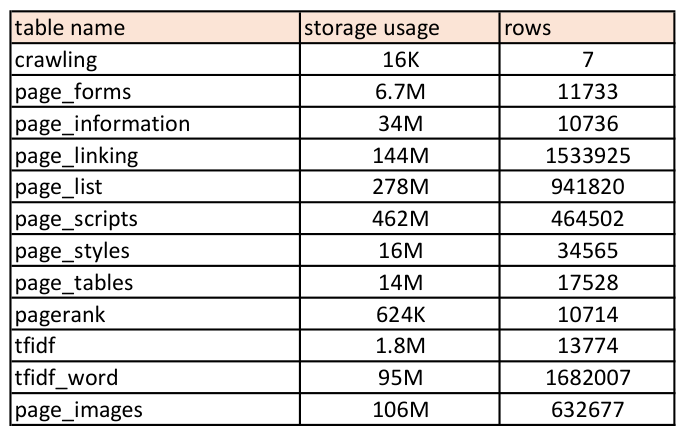
\includegraphics[keepaspectratio, width=12cm]{gambar/db-usage.png}
%		\caption{Penggunaan storage masing masing tabel dalam database}}
%	\label{gambar:db-usage.png}
%\end{figure}


\section{Celery}

Celery merupakan \textit{framework task queue} yang ditulis dengan menggunakan bahasa pemrograman \textit{python}. Program \textit{Celery} dapat membantu menangani tugas tugas yang berkaitan dengan mengatur pembagian kerja dalam beberapa pekerja.


\section{Mongo DB}
MongoDB dikembangkan pada tahun 2007 oleh Eliot dan Dwight untuk 10gen, yang merupakan sistem basis data yang berbasis dokumen yang dapat berjalan di berbagai platform. MongoDB termasuk basis data yang jatuh pada kategori NoSQL. Salah satu alasan dibuatnya MongoDB adalah kemampuan manajemen data dalam jumlah besarnya \citep{mongoarchitecture}.  MongoDB menyimpan dokumen dalam bentuk seperti JSON atau \textit{Javascript Object Annotation} yang bentuknya dapat bermacam macam. Informasi yang relevan dapat disimpan secara bersama sama untuk \textit{query} dengan akses yang cepat dengan \textit{MongoDB query language}. MongoDB menggunakan skema yang dinamis yang membantu dalam membuat \textit{record} tanpa mendefinisikan strukturnya terlebih dahulu seperti atribut atau tipe data. MongoDB memungkinkan untuk mengubah struktur data dengan mudah dengan cara menambahkan atribut atau menghapus atribut yang ada. Model penyimpanan seperti ini membuat membantu dalam merepresentasikan hubungan hierarki, menyimpan data \textit{arrays} dan struktur yang kompleks lainnya dengan mudah. Sebuah dokumen dalam suatu \textit{record} tidak diharuskan memiliki atribut yang sama. MongoDB dirancang untuk availabilitas tinggi dan skalabilitas yang termasuk \textit{replication} dan \textit{auto-sharding} \citep{mongoarchitecture2}.

MongoDB mendukung dua tipe replikasi yaitu \textit{master-slave} dan \textit{replica sets}. Dalam replikasi \textit{master-slave}, \textit{master} mempunyai akses data penuh dan menentukan siapa yang berhak menulis setiap perubahan kepada \textit{slave}. Para \textit{slave} dalam tipe replika ini hanya dapat membaca data saja. Untuk \textit{replica sets}, memiliki cara kerja yang sama dengan replikasi \textit{master-slave}, akan tetapi \textit{replica sets} memungkinkan untuk memilih \textit{master} yang baru jikalau \textit{master} yang lama tidak dapat melakukan kewajibannya. Fitur lainnya yang didukung oleh MongoDB adalah \textit{automatic sharding}. Dengan menggunakan fitur ini, data dapat dibagi-bagi ke beberapa \textit{node}. Seseorang harus memverfikasi \textit{sharding key} untuk setiap \textit{collection} yang mendefiniskan bagaimana suatu dokumen dapat dibagi-bagi. \citep{mongoarchitecture2}

\begin{figure}[H]
	\centering
	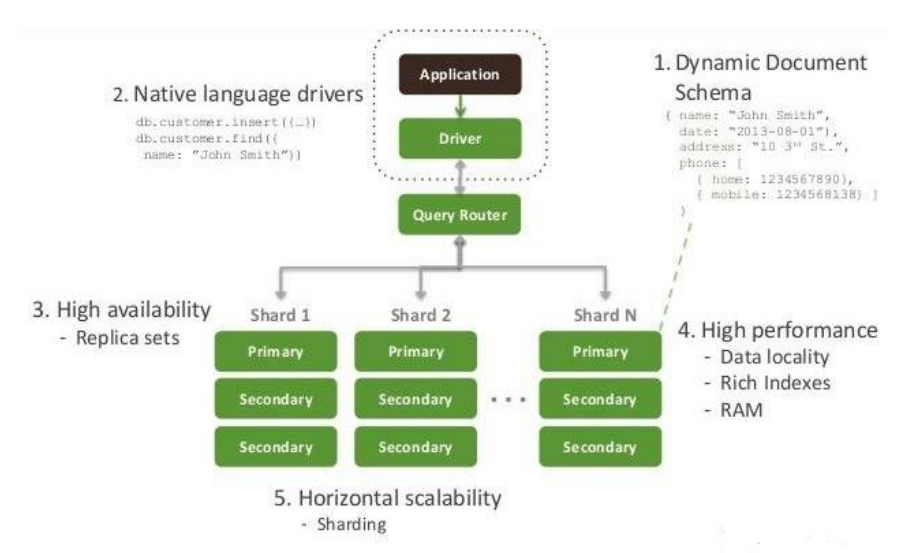
\includegraphics[keepaspectratio, width=16cm]{gambar/arsitektur-mongodb}
	\caption{Arsitektur MongoDB}
	\label{gambar:arsitektur-mongodb}
\end{figure}

Pada umumnya dalam arsitektur MongoDB terdapat beberapa komponen pendukung seperti:
\begin{enumerate}
	\item{\emph{Configuration Servers} bertugas untuk menyimpan metadata dari \textit{sharded cluster}. Data yang disimpan mengandung informasi berupa \textit{mapping dataset cluster} dengan \textit{shard}. Komponen seperti \textit{query router} menggunakan data ini untuk menargetkan operasi yang datang ke shard yang sesuai.} 
	\item{\emph{Query Routers}  berhadapan langsung dengan aplikasi dan mengalihkan operasi ke shard atau shards yang sesuai.} 
	\item {\emph{Shards} menyimpan data dan memberikan availabilitas dan konsistensi data yang tinggi.}
\end{enumerate}

Dibandingkan dengan MySQL, MongoDB lebih baik dalam hal pemrosesan query \citep{mongoarchitecture2}. Hal ini dibuktikan dengan penelitian yang bertujuan untuk melihat kelebihan antara penggunaan database non-relasional MongoDB dengan database relasional MySQL. Pada penelitian ini dilakukan beberapa operasi basik kepada kedua database yaitu MongoDB dan MySQL. Operasi yang dilakukan yaitu \textit{insert}, \textit{select}, \textit{update} dan \textit{delete}. Penelitian dilakukan dengan perangkat keras seperti Windows 7
Ultimate 64-bit, prosessor Intel Core i3 (2.4 GHz), 4 GB RAM memory. Sebelum penelitian dilakukan kedua database memiliki beberapa tabel denngan skema yang sama yaitu:

\begin{enumerate}
	\item{tabel/dokumen \textit{User} dengan kolom id, username,
		password, email.}
	\item{tabel/dokumen \textit{Forum} dengan kolom: id, title,
		author, info (short description).}
	\item{tabel/dokumen \textit{Subforum} denga kolom: id, title,
		author, info, created, updated.}
	\item{tabel/dokumen \textit{Discussion} dengan kolom: id, title,
		author, created, updated, content. }
	\item{tabel/dokumen \textit{Comments} dengan kolom: id, author,
		created, content, approved. }
\end{enumerate}

Pemasukan data dimulai dengan memasukan data pengguna ke kedua database, 10.000 pengguna dimasukan ke dalam dua database. Untuk id user dihasilkan secara automatis oleh kedua database dan untuk atribut seberti \textit{username}, \textit{password} dan alamat \textit{email} digunakan fungsi PHP seperti \textit{md5}, \textit{rand}, \textit{substr} dan \textit{str shuffle}. Setelah pemasukan data dilakukan, MySQL memerlukan waktu selama 440 detik sedangkan MongoDB memerlukan waktu sekitar 0.29 detik. Untuk pengujian performa \textit{query} data data dalam jumlah besar, terlihat MongoDB lebih performan daripada MySQL.

\begin{figure}[H]
	\centering
	\includegraphics[keepaspectratio, width=12cm]{gambar/2-grafik-mongomysql-1}
	\caption{Perbandingan performa pemasukan data pengguna untuk kedua database}
	\label{gambar:2-grafik-mongomysql-1}
\end{figure}

Ketika semua pengguna berhasil dimasukan kedalam database, pemasukan data dilanjutkan dengan pemasukan data forum, subforum, diskusi dan komentar. Untuk pengujian, dilakukan pemasukan 5000 baris data untuk setiap tabel forum, subforum, diskusi, dan komentar. Setelah pemasukan data dilakukan, MySQL memerlukan waktu selama 1010 detik sedangkan MongoDB memerlukan waktu sekitar 3.3331 detik. Ketika semua pengguna berhasil dimasukan kedalam database, pemasukan data dilanjutkan dengan pemasukan data forum, subforum, diskusi dan komentar. Untuk pengujian, dilakukan pemasukan 5000 baris data untuk setiap tabel forum, subforum, diskusi, dan komentar. Setelah pemasukan data dilakukan, MySQL memerlukan waktu selama 1010 detik sedangkan MongoDB memerlukan waktu sekitar 3.3331 detik. Untuk pengujian performa untuk pemasukan data dalam jumlah besar, terlihat MongoDB lebih performan daripada MySQL dalam hal memasukan data yang besar.

Selanjutnya adalah pengujian operasi \textit{query}, diadakan dua operasi \textit{query} yaitu:
\begin{enumerate}
	\item {\textit{Query} pertama untuk semua diskusi yang suatu user lakukan dan dengan tanggal yang berbeda dari yang ditentukan.}
	\item {\textit{Query} kedua untuk semua pengguna dari database dan jumlah diskusi yang dimulai oleh setiap user}
\end{enumerate}

\begin{figure}[H]
	\centering
	\includegraphics[keepaspectratio, width=12cm]{gambar/2-grafik-mongomysql-2}
	\caption{MySQL vs MongoDB Select}
	\label{gambar:2-grafik-mongomysql-2}
\end{figure}

Dari tabel diatas, untuk operasi query yang pertama, MySQL memerlukan waktu sekitar 0.0018 detik sedangkan MongoDB berhasil dieksekusi dalam waktu 0.0011 detik dan untuk operasi yang kedua, MySQL memerlukan waktu sekitar 0.6478 detik dan MongoDB memerlukan waktu 0.0052 detik. Untuk pengujian performa untuk query data dalam jumlah besar, terlihat MongoDB lebih performan daripada MySQL dalam hal melakukan operasi \textit{query}.

Selanjutnya adalah pengujian operasi \textit{update} database, ada dua operasi \textit{update} yang digunakan dalam pengujian ini:
\begin{enumerate}
	\item{Mengupdate suatu komen yang ditulis oleh suatu user}
	\item{Mengupdate alamat email suatu pengguna}
\end{enumerate}

\begin{figure}[H]
	\centering
	\includegraphics[keepaspectratio, width=12cm]{gambar/2-grafik-mongomysql-3}
	\caption{MySQL vs MongoDB update}
	\label{gambar:2-grafik-mongomysql-3}
\end{figure}

Untuk operasi update yang pertama, MySQL memerlukan waktu sekitar 0.0987 detik sedangkan dalam MongoDB operasi query update yang pertama dilakukan dalam 0.0428 detik. Untuk pengujian performa untuk update data dalam jumlah besar, terlihat MongoDB lebih performan daripada MySQL dalam hal melakukan operasi \textit{update}.

Selanjutnya dilakukan pengujian untuk operasi \textit{delete}. Ada dua operasi \textit{delete} yang dilakukan untuk pengujian yaitu:
\begin{enumerate}
	\item{Menghapus semua forum yang dibuat oleh suatu user}
	\item {Menghapus semua komentar yang dibuat oleh suatu user.}
\end{enumerate}

\begin{figure}[H]
	\centering
	\includegraphics[keepaspectratio, width=12cm]{gambar/2-grafik-mongomysql-4}
	\caption{MySQL vs MongoDB delete }
	\label{gambar:2-grafik-mongomysql-4}
\end{figure}

Dari gambar \ref{gambar:2-grafik-mongomysql-4}, MySQL memerlukan waktu sekitar 0.3524 detik, sedangka MongoDB memerlukan 0.0028 detik dan operasi yang kedua, MySQL memerlukan waktu 0.8231 detik dan MongoDB memerlukan waktu sekitar 0.0064 detik.

MongoDB memberikan waktu eksekusi operasi yang lebih rendah dibandingkan dengan MySQL dalam 4 operasi biasa yang dimana hal ini adalah hal yang penting ketika sebuah aplikasi diharuskan mendukung ribuan pengguna secara bersama-sama. Maka dari itu dari penelitian yang dilakukan sebelumnya, MongoDB mempunyai performa yang baik dan lebih dipilih dibandingkan MySQL \citep{mongomysqlperfomancediff}.




% Baris ini digunakan untuk membantu dalam melakukan sitasi
% Karena diapit dengan comment, maka baris ini akan diabaikan
% oleh compiler LaTeX.
\begin{comment}
\bibliography{daftar-pustaka}
\end{comment}

